%%% PLANTILLA DISEÑADA PARA LA REALIZACIÓN DE TESIS DE GRADO DE LA UNIVERSIDAD NACIONAL DEL CALLAO
%% AUTOR DE LA PLANTILLA: RODOLFO ZEVALLOS SALAZAR

\documentclass[spanish,12pt,a4paper,twoside,openright]{report}


\usepackage[T1]{fontenc}
\usepackage{times}
\usepackage[utf8]{inputenc}
\usepackage{amsmath}
\usepackage{graphicx}
\usepackage{multicol}
\usepackage{longtable}
\usepackage[refpages]{gloss}
\usepackage{float}
\usepackage{anysize}
\usepackage{appendix}
\usepackage{lscape} 
\usepackage{pdflscape}
\usepackage{multirow}
\usepackage{listings}
\usepackage{color}
\usepackage{setspace}
\usepackage{enumerate} 
\usepackage{placeins}
\usepackage{graphics}
\usepackage{enumitem}
\usepackage{caption}


\usepackage{hyperref}
\hypersetup{
	colorlinks,
	citecolor=black,
	filecolor=black,
	linkcolor=black,
	urlcolor=black
}

\usepackage[textwidth=15cm, textheight=22.5cm, top=0.5cm, bottom=3.5cm,left= 3cm,right=3cm]{geometry}

\usepackage{babel} 
\usepackage{apalike}

\usepackage{apacite}
\usepackage[nottoc,numbib]{tocbibind} %Para la bibliografia

\usepackage{fancyhdr}

\pagestyle{fancy}
\fancyhf{}
%\fancyhead[LE,RO]{Overleaf}
\fancyhead[RE,LO]{\leftmark}
\fancyfoot[CE,CO]{Abel de Andrés Gómez}
\fancyfoot[LE,RO]{\thepage}

\renewcommand{\headrulewidth}{2pt}
\renewcommand{\footrulewidth}{1pt}

\usepackage{tocloft}
\setlength{\cftchapnumwidth}{20pt}  % Width of section No

%para los chapter
\usepackage{titlesec, blindtext, color}
\definecolor{gray75}{gray}{0.75}
\newcommand{\hsp}{\hspace{20pt}}
\titleformat{\chapter}[hang]{\Huge\bfseries}{\thechapter\hsp\textcolor{gray75}{|}\hsp}{0pt}{\Huge\bfseries}

\titlespacing*{\chapter}{0pt}{-50pt}{20pt}

%\usepackage[hyphens]{url} %Para las URL de la bibliografia
\usepackage{verbatim} % comentarios

\newcommand\blankpage{%
	\null
	\thispagestyle{empty}%
	\addtocounter{page}{-1}%
	\newpage}

\pagenumbering{gobble}

\begin{document}

%----------------------------------------------------------------------------------------
%	CONFIGURACION
%----------------------------------------------------------------------------------------


\renewcommand*{\contentsname}{ÍNDICE}
\renewcommand*{\listtablename}{Índice de tablas}
\renewcommand*{\listfigurename}{Índice de figuras}
\renewcommand{\baselinestretch}{1.5}
\renewcommand{\appendixname}{ANEXOS}
\renewcommand{\appendixtocname}{ANEXOS}
\renewcommand{\appendixpagename}{ANEXOS}
\renewcommand{\thetable}{\arabic{chapter}.\arabic{table}}
\renewcommand*{\tablename}{Tabla}
\renewcommand*{\chaptername}{Capítulo}
\renewcommand*{\thechapter}{\arabic{chapter}}
\renewcommand{\thesection}{\arabic{chapter}.\arabic{section}}
\renewcommand{\figurename}{Figura}
\renewcommand{\thefigure}{\arabic{chapter}.\arabic{figure}}
\renewcommand{\theequation}{\arabic{chapter}.\arabic{equation}}
\renewcommand{\BOthers}[1]{et al.\hbox{}}%para poner el et.al



%----------------------------------------------------------------------------------------
%	PORTADA
%----------------------------------------------------------------------------------------

\begin{titlepage}
	
	\newcommand{\HRule}{\rule{\linewidth}{0.5mm}} % Defines a new command for the horizontal lines, change thickness here
	
	%\renewcommand{\baselinestretch}{1.5}
	
	
	%Separacion de los listados
	%\setlist[itemize,2]{topsep=0mm}
	%\setlist[itemize]{itemsep=0pt,topsep=0pt,partopsep=0pt}
	%\setenumerate{itemsep=0pt,topsep=0pt}
	%\SetEnumitemKey{midsep}{topsep=0pt, partopsep=0pt}
	
	
	\center % Center everything on the page
	\vspace*{0pt}
	\textsc{\huge Universidad Rey Juan Carlos }
	\\[1cm]
	
	% HEADING SECTIONS
	%
\includegraphics[width=2.25cm]{recursos/logoFi.png}
	
\includegraphics[width=6cm]{recursos/escudo_urjc}
	\\[1cm]
	
	\textsc{\Large Trabajo Fin de Máster }\\[0.2cm]
	% TITLE SECTION
	\HRule \\[0.4cm]
	{ \Huge \bfseries Explotación y modelos para predicción de datos en el Sistema Educativo de la Comunidad de Madrid}\\[0.2cm] % Title of your document
	\HRule \\[1cm]
	
	\textsc{\Large Máster Universitario En Formación del Profesorado de Ed.Secundaria, Bachillerato, FP e Idiomas }\\[0.7cm]
	\textsc{\Large Especialidad en Informática y Tecnología }\\[1cm]
	\textsc{\Large Curso 2018-2019}\\[1cm]
	
	% AUTHOR SECTION
	\begin{flushright}
		\large
		AUTOR: Abel de Andrés Gómez\\
		DIRECTOR: Aurelio Berges García\linebreak
	\end{flushright}
	
	%\vspace{1cm}
	
	\vfill % Fill the rest of the page with whitespace
	
\end{titlepage}
\newgeometry{textwidth=15cm, textheight=22.5cm, top=3.5cm, bottom=3.5cm,left= 3cm,right=3cm}
\blankpage

%----------------------------------------------------------------------------------------
%	Dedicatoria
%----------------------------------------------------------------------------------------
\begin{comment}
\begin{titlepage}

\begin{flushright}
{\large \bf DEDICATORIA}
\\
\textit{}
\\
\textit{} % agregar tu dedicatoria
\end{flushright}
\end{titlepage}
\blankpage
\end{comment}

%----------------------------------------------------------------------------------------
%	Agradecimientos
%----------------------------------------------------------------------------------------

\begin{titlepage}

\begin{flushright}
{\large \bf AGRADECIMIENTOS}
\vspace{10pt}

{\normalsize Desde estas lineas me gustaría expresar mi mas sincero agradecimiento: \newline
	
A mi tutor Aurelio Berges, por ayudarme y guiarme durante todo el proyecto.
\newline

A Felipe Retortillo, por ayudarme con toda la información necesaria para realizar este TFM.
\newline

A mis padres, por haberme proporcionado la mejor educación y lecciones de vida.
\newline

En especial a mi padre, por haberme enseñado que, con esfuerzo, trabajo y constancia todo se consigue, y que en esta vida nadie regala nada.
\newline

En especial a mi madre, por hacerme ver cada dia la vida de una forma diferente y confiar en mis decisiones. Sin olvidar su infinita ayuda durante estos últimos años.
\newline

A todos mis familiares por haberme apoyado y animado.
\newline

A mis compañeros del máster, con los que he compartido buenos momentos a lo largo de las intensas tardes del máster.
\newline

A mis amigos, por estar siempre a mi lado.
\newline

A todos aquellos que siguen estando cerca de mi y que le regalan a mi vida algo de ellos.}
% agregar tu dedicatoria
\end{flushright}
\end{titlepage}
\blankpage

%----------------------------------------------------------------------------------------
%	RESUMEN
%----------------------------------------------------------------------------------------

\begin{titlepage}
	
	\begin{flushright}
		{\large \bf RESUMEN}
		\\
		\vspace{10pt}
		\textit{}
		{La planificación de grupos escolares es una tarea complicada que debe realizar la Consejería de Educación e Investigación de la Comunidad de Madrid. Gestionar los recursos de la mejor forma es vital para mejorar la calidad educativa. Por tanto, se hace necesario el estudio de las variables más importante que permitan un mejor reparto de los medios disponibles.
	%Las lesiones traumáticas cerebrales son un problema de salud mundial. Por tanto, se hace necesario el estudio de los predictivos considerados medicinalmente más importantes. El motivo es establecer estrategias, decisiones clínicas y protocolos para el tratamiento de estas lesiones de forma óptima y tratando siempre de obtener el mejor resultado en el paciente.
	
	En los estudios que se realizan se utilizan datos de los grupos actuales de distintos centros, entre otras variables. Con esta información se han construido varios modelos que permitan predecir el número de grupos que deben planificarse para el curso siguiente y poder así repartir los recursos disponibles (profesores, suministros, etc.).
	
	En este estudio se realiza una clasificación sobre la importancia de las variables existentes, además se realizan estudios estadísticos para obtener la relación que existen entre estas variables para posteriormente utilizar distintos modelos con el objeto de conseguir la mayor predicción posible.
	
	Para obtener el mejor modelo se utilizan distintas métricas con el objetivo de poder compararlos entre sí en función de las necesidades que se requieran.

		} % agregar tu dedicatoria
	\end{flushright}
\end{titlepage}
\blankpage
%----------------------------------------------------------------------------------------
%	ABSTRACT
%----------------------------------------------------------------------------------------

\begin{titlepage}
	
	\begin{flushright}
		{\large \bf ABSTRACT}
		\\
		\textit{}
		{} % agregar tu dedicatoria
	\end{flushright}
\end{titlepage}
\blankpage

%----------------------------------------------------------------------------------------
%	TABLA DE CONTENIDOS
%---------------------------------------------------------------------------------------
\pagenumbering{roman} 

\tableofcontents
\cleardoublepage
\listoftables
\listoffigures 
\makegloss
\newpage


%----------------------------------------------------------------------------------------
%	Resumen
%----------------------------------------------------------------------------------------

%\chapter*{\centering \large RESUMEN} % si no queremos que añada la palabra "Capitulo"
%\addcontentsline{toc}{section}{RESUMEN} % si queremos que aparezca en el índice
%\markboth{RESUMEN}{RESUMEN} % encabezado
%\doublespacing

%----------------------------------------------------------------------------------------
%	Abstract
%----------------------------------------------------------------------------------------

%\chapter*{\centering \large ABSTRACT}
%\addcontentsline{toc}{section}{ABSTRACT}
%\markboth{ABSTRACT}{ABSTRACT}


%----------------------------------------------------------------------------------------
%	INTRODUCCIÓN
%----------------------------------------------------------------------------------------

\pagenumbering{arabic} 
\onehalfspacing
\setlist[itemize,2]{topsep=0mm}
\setlist[itemize]{itemsep=-5pt,topsep=0pt,partopsep=0pt}
\setenumerate{itemsep=0pt,topsep=5pt,partopsep=-5pt}
%\marginsize{3.0cm}{3.0cm}{0.0cm}{3.0cm}


%\chapter*{\centering \large INTRODUCCIÓN} % si no queremos que añada la palabra "Capitulo"
%\addcontentsline{toc}{section}{INTRODUCCIÓN} % si queremos que aparezca en el índice
%\markboth{INTRODUCCIÓN}{INTRODUCCIÓN} % encabezado

\chapter{Introducción}
\section{Introducción}
Uno de los problemas que se plantea en la actualidad en el proceso de enseñanza-aprendizaje es la cantidad de alumnos que están en una misma aula a cargo de un solo docente. Este aspecto es uno de los más debatidos en la educación. \cite{PANORAMA2018}

Según \citeA{LILIA2013}, la superpoblación estudiantil es el exceso del número de estudiantes que se encuentran en un espacio determinado cuya capacidad no es adecuada para acogerlos ni cuenta con las condiciones adecuadas para el buen desenvolvimiento de los mismos.

En el caso particular de España, el tamaño de clase medio en Educación Secundaria en las instituciones públicas es superior al promedio de la OCDE y de la UE22. \cite{PANORAMA2018}

Esto no implica que en todos los casos en el que la ratio sea superior exista una sobrepoblación, sin embargo, la calidad educativa se ve mermada por esta situación.

\begin{figure*}[htb]
	\centering
	\caption{Número medio de alumnos por clase en instituciones públicas (2016). Recuperado del \protect\citeA{PANORAMA2018}}
	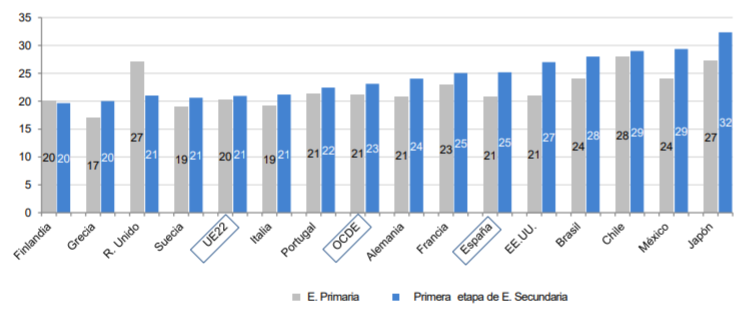
\includegraphics[width=0.8\textwidth]{recursos/NumeroAlumnosClase}
	\label{fig:NumeroAlumnosClase}
\end{figure*}
\FloatBarrier

En la figura \ref{fig:NumeroAlumnosClase} se puede observar como la media del número de alumnos por clase de la Unión Europea está en 21 alumnos para la etapa de Secundaria, mientras que en España la media asciende a 25 alumnos.

Si bien es cierto, que es bueno que se deba atender a la diversidad y a la inclusión (sobre el número de alumnos) en el aula, esto debe hacerse de forma responsable y conociendo las limitaciones que tiene el docente, que por más voluntad o capacitación que posea, tiene que atender a las necesidades personalizadas de cada alumno. \cite{HILDA2014}

\citeA{lera2007calidad} en su articulo se plantea la reducción del numero de alumnos o el aumento de asistentes en el aula con el objetivo de mejorar la calidad educativa. 

La ratio, que es la relación entre el número de alumnos y profesores, es un factor importante a la hora de realizar la planificación de los recursos. En el año 2012, dicho ratio, en España aumentó un 20\%, lo que implica un ahorro en torno a 464 millones de euros. Aprobado por el Real Decreto-ley 14/2012 en el artículo 2.

Debido a que los recursos de una administración no son infinitos, es necesario tener en cuenta los recursos disponibles para la educación; concretamente, durante 2015 España presenta un gasto total por alumno inferior al promedio de los países de la OCDE y la UE22. Véase la figura \ref{fig:procPerformance}. Esto implica que se dispone de menos recursos en la educación y por lo tanto se tiende a agrupar a los alumnos en grupos de mayor tamaño.

\begin{figure*}[htb]
	\centering
	\caption{Gasto total anual (2015). Recuperado del \protect\citeA{PANORAMA2018}}
	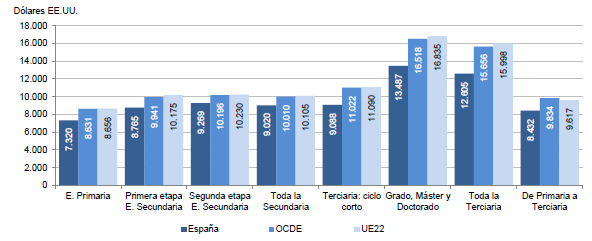
\includegraphics[width=0.8\textwidth]{recursos/GastoEducacion}
	\label{fig:procPerformance}
\end{figure*}
\FloatBarrier

Por las razones anteriormente comentadas, es importante establecer una buena gestión sobre los recursos disponibles, realizando una óptima distribución tanto de los docentes como de los recursos asignados a estos.

\begin{comment}
En los últimos años, gracias al gran desarrollo tecnológico que se ha vivido tanto a nivel de computo (mejorando la eficiencia y el uso de los recursos disponibles) como a nivel de transmisión de datos (mejorando las comunicaciones), ha permitido a las organizaciones el almacenamiento de una gran cantidad de información.

Para comprender mejor este gran volumen de información que disponen las organizaciones, es necesario utilizar métodos, técnicas, herramientas además de personas con conocimientos (formando todas esta un vínculo estrecho) que permita y ayude a explotar, investigar, predecir y obtener información relevante para tomar decisiones de forma adecuada.

Para descubrir la información en estos grandes volúmenes de datos, es necesario abordar el concepto de minería de datos.  Según \citeA{martinez2016mineria}, la minería de datos es el ``proceso que permite transformar información en conocimiento útil para el
negocio, a través del descubrimiento y cuantificación de relaciones en una
gran base de datos". La minería de datos aplica técnicas estadísticas y matemáticas para poder obtener esta información implícita en los datos.

Algunas de las aplicaciones de la minería de datos según \cite{riquelme2006mineria} son:  comercio y banca, medicina y farmacia, seguridad y detección de fraude, astronomía, geología, minería, agricultura, pesca, ciencias ambientales y ciencias sociales.


\section{Contexto}
Las organizaciones de ámbito educativo no han quedado ajenas a estas necesidades de una mejor comprensión de los datos. Según \citeA{romero2010educational} la minería de datos educativa (EDM) se encarga del desarrollo de métodos para explotar los datos del entorno educativo y entender mejor a los estudiantes y las herramientas que se utilizan para el aprendizaje de estos.

Por un lado, tanto el software educativo como las bases de datos institucionales, han generado una gran cantidad de datos acerca de alumnos, reflejando el aprendizaje de estos a lo largo del tiempo. Por otro, el uso pedagógico de Internet (eLearning), ha generado también grandes cantidades de datos acerca de la enseñanza-aprendizaje (técnicas, herramientas, etc). "Toda esta información es una mina de oro, en el contexto educativo". \cite{romero2010educational}.

\citeA{MOHAMAD2013320} define EDM como una disciplina emergente, relacionada con el desarrollo de métodos para la explotación de datos que proceden del entorno educativo, para entender mejor a los estudiantes y las herramientas que estos utilizan para aprender. Coincide con el artículo de \citeA{inbook} en el que se indica que la EDM se ha desarrollado más lentamente que en el resto de ámbitos.

Como se puede observar en el artículo de \citeA{sin2015application} y en la figura \ref{fig:artPublicados}, el número de artículos publicados en la conferencia internacional sobre la minería de datos ha crecido desde 2011 casi exponencialmente.

Este aumento de artículos publicados muestra como existe un aumento en el uso de la minería de datos en la educación.

\begin{figure*}[htb]
	\centering
	\caption{Artículos aceptados y publicados desde 2011. Recuperado de \protect\citeA{sin2015application}}
	\includegraphics[width=0.6\textwidth]{recursos/artPublicados}
	\label{fig:artPublicados}
\end{figure*}
\FloatBarrier

A su vez, \citeA{sin2015application}, ha categorizado los artículos publicados según su contenido en categorías que definen las distintas aplicaciones de la minería de datos en la educación. Algunas de estas categorías son: detección de comportamiento, estimación de habilidades, predicción de mejora académica, etc. Por tanto, como se puede observar, dentro de la minería de datos en el entorno educativo, existen distintos campos estudiados y distintos ámbitos de aplicación.
\end{comment}

\section{Objetivos} 
\label{objetivos}
En este trabajo fin de máster (TFM) se expone una solución a la necesidad que tiene la Consejería de Educación e Investigación de la Comunidad de Madrid (CEI) para dar respuesta a las necesidades de la demanda concreta de plazas escolares de un nuevo período escolar. Para ello, se plantea el uso de herramientas y métodos flexibles que automaticen las tareas de planificación y proponga, además, nuevas variables o factores que puedan influir en la toma de decisiones. 

El interés que justifica este TFM es avanzar en el conocimiento sobre los factores del entorno educativo que implican el aumento de la superpoblación de un aula. De esta manera, se consigue que las Unidades (que tienen la competencia de gestionar la demanda de plazas escolares de un nuevo periodo escolar) tengan mayor facilidad a la hora de implantar un Sistema que sea capaz de predecir el número de grupos, a partir de los factores disponibles en cursos previos.

Las consideraciones que se han realizado en los párrafos anteriores justifican que el objetivo general de este TFM es: proponer un modelo para contribuir a la óptima planificación de los grupos escolares para los nuevos cursos, evitando así el gasto innecesario de recursos y controlando la sobrepoblación en el aula.

Dicho objetivo global se pretende alcanzar mediante los siguientes sub objetivos:
\begin{itemize}
	\item Seleccionar variables de interés, relativas a la resolución de la necesidad anteriormente expuesta por Unidad de Planificación, que aporten valor en el desarrollo de este TFM. 
	\item Estudiar la relación entre dichas variables con el propósito de comprender el contexto de la sobrepoblación en el aula y la planificación de grupos.
	\item Probar distintos modelos predictivos y seleccionar aquellos que aporten mayor precisión en la predicción de los grupos. 
	\item Obtener y utilizar el modelo de mayor precisión para realizar predicciones con los datos existentes en el entorno educativo de la Comunidad de Madrid en los últimos 10 años y que este modelo ayude a las Unidades de la CEI a planificar grupos en los nuevos cursos. 
\end{itemize}

\section{Metodología}
El proceso o metodologia llevado a cabo en este TFM sigue las siguientes fases:
\begin{enumerate}
	\item En primer lugar, se detecta la necesidad ya expuesta por la Unidad de la Consejería de Educación e Investigación de la Comunidad de Madrid\footnote{El autor de este TFM ha colaborado con la Consejería de Educación e Investigación de la Comunidad de Madrid en el desarrollo de un proyecto (ALAS) sobre explotación de datos educativos coordinado por la Universidad Politécnica de Madrid, a lo largo del año 2018.}.
	\item Una vez detectada la necesidad, se realizan reuniones con dicha Unidad para obtener la máxima información posible acerca de las necesidades concretas y la forma de satisfacerlas. \footnote{Antes de comenzar la investigación, se debe tener un claro conocimiento sobre las necesidades existentes y se debe establecer un plan de acción.}
	\item Teniendo en cuenta el conocimiento sobre cuáles son las necesidades, se realiza una propuesta\footnote{Esta propuesta es un documento técnico donde se indica qué metodologías se van a emplear para llevar a cabo la investigación, qué modelos predictivos se van a considerar y fundamentalmente cuales son las variables que se van a usar en la predicción (teniendo en cuenta las necesidad de la Unidad de Planificación).} que incluya modelos, variables, y herramientas a la Unidad de Planificación para poder satisfacerlas.% una propuesta que incluya ...
	\item Después de varias reuniones con la Unidad de Planificación, esta Unidad valida la propuesta.
	\item Una vez validada la propuesta, se estudian distintos modelos de predicción a partir de los datos seleccionados en dicha propuesta. Se debe analizar cuál de estos modelos es el que mayor precisión obtiene.
	\item Se decide, en una reunión con la Unidad de Planificación de Centros, cual es el modelo óptimo (teniendo en cuenta la precisión y el tiempo de entrenamiento de los modelos). 
	\item A partir del modelo acordado, se realizan predicciones con los datos de la Unidad.
\end{enumerate}

\section{Organización del TFM}
La estructura que se va a seguir en el TFM es la siguiente:
\begin{itemize}
	\item \textbf{Capítulo 1. Introducción:} En el primer capítulo se definen las necesidades existentes que justifican el desarrollo de este trabajo. También se definen los objetivos que se persiguen con el desarrollo de este. Por último, se presenta la estructura que tiene el presente documento.
	\item \textbf{Capítulo 2. Justificación teórica:} En este segundo capítulo se realiza una investigación sobre el estado de la cuestión, estudiando los métodos, modelos y usos de la minería de datos en el ámbito educativo. 
	\item \textbf{Capítulo 3. Propuesta de intervención:} En este capítulo se define el problema existente.
	\item \textbf{Capítulo 4. Diseño de la investigación:} Este capítulo establece los pasos que se siguen en la realización de un proyecto de minería de datos. Se detallan también las tareas que se van a desempeñar en cada uno de los pasos.
	\item \textbf{Capítulo 5. Análisis de los resultados:} Una vez realizado el análisis exploratorio y predictivo, se mostrarán los resultados obtenidos en este capítulo.
	\item \textbf{Capítulo 6. Conclusiones:} En este capítulo se detallan las conclusiones obtenidas a partir de los resultados alcanzados y los objetivos establecidos.
\end{itemize}


%----------------------------------------------------------------------------------------
%	PLANTEAMIENTO DE LA INVESTIGACIÓN
%----------------------------------------------------------------------------------------


\section{JUSTIFICACIÓN TEÓRICA}
\subsection{Introducción}
%https://www.thetechedvocate.org/8-ways-machine-learning-will-improve-education/

Uno de los intereses que se tienen a la hora de realizar cualquier proyecto de ``Big Data'', ``Business Intelligence'' o un análisis predictivo son las variables a utilizar, ya que son las que van a permitir obtener la mayor información esperada.

Esta investigación se realiza con el propósito de aportar conocimiento existente sobre la importancia de determinadas variables educativas y su relevancia en la predicción, la planificación y la gestión educativa. 

Para ello, y, teniendo en cuenta los propósitos de esta investigación, se debe establecer el objeto de búsqueda de documentación científica acerca de la minería de datos en el ámbito educativo, más concretamente, en la educación secundaria. 

A partir del objeto de búsqueda, se debe establecer las fuentes que se utilizan para obtener resultados fiables, ya que en la actualidad existen numerosos artículos acerca del uso de la ciencia de datos, pero es necesario acotar la búsqueda a lo relativo a educación.

Para la realización de este TFM se han analizado distintas publicaciones de la base de datos científica de Web of Science. 

Para realizar la búsqueda se han utilizado las siguientes palabras clave: ``educational", ``data'' y ``mining". Se debe recordar que el éxito de la búsqueda depende de estas palabras claves. También se ha realizado una búsqueda utilizando estas claves en Teseo, ScienceDirect y Google Academics.

De la búsqueda en ``Web of Science'' con las claves comentadas se han obtenido un gran número de publicaciones. Por tanto, se ha tenido que acotar la búsqueda incluyendo nuevas palabras claves (``models'' y ``predictions''). De esta nueva búsqueda se han obtenido 47 artículos. Posteriormente se ha realizado una observación sobre los artículos obtenidos y se ha comprobado la existencia de artículos que no resultan útiles en esta investigación, por lo que se han descartado.

Además, de la primera búsqueda, donde se obtenían gran cantidad de resultados, se han revisado, entre otros, los artículos más populares (respecto a su número de citas) y actuales, y se han seleccionado 15 que se ajustan a las necesidades de este estudio.

Complementariamente, también se ha realizado búsquedas incluyendo la clave de ``gis". El motivo de esta búsqueda es intentar encontrar artículos centrados en GIS (Sistemas de Información Geográfica). Los sistemas de información geográfica, como su propio nombre indica, se utilizan para referenciar datos en el espacio. 


%De la búsqueda en ScienceDirect se han obtenido 160 artículos. Posteriormente se han tenido en cuenta aquellos de los últimos 5 años (2015, 2016, 2017, 2018 y 2019), sin olvidarse del resto. De esta forma obtenemos resultados actuales (concretamente 73 artículos). Posteriormente se ha realizado una observación sobre los artículos obtenidos y se ha comprobado la existencia de artículos que no resultaban útiles en esta investigación. Por tanto, se ha realizado otra búsqueda utilizando las claves anteriores y añadiendo la clave "prediction". Esta vez, se han obtenido 26 resultados. De todos los resultados obtenido, se han seleccionado 15 artículos que se consideran útiles y que servirán de ayuda.

Debemos destacar que la mayoría de los resultados obtenidos tratan de artículos centrados en la predicción de los resultados académicos de los alumnos teniendo en cuenta ciertos factores internos (como las propias calificaciones a lo largo del curso) y externos (como factores etnográficos, edad, situación económica familiar, etc.). Estos factores se han utilizado principalmente para obtener una aproximación sobre las calificaciones, y el fracaso escolar. Mostrando de forma implícita las relaciones de estos aspectos con el resultado (calificación).

%AMPLIAR UN POCO ESTO, ES LO MAS IMPORTANTE

%En este sentido es interesante realizar un análisis de dichos artículos, puesto que en primer lugar se deberá tener en cuenta cuales son las metodologías de la ciencia de datos que se están utilizando. Además, en segundo lugar, se debe tener en cuenta los modelos que se utilizan para predecir variables de carácter educativo. 

%Una vez que se han analizado los artículos, se ha decido realizar otra búsqueda en ScienceDirect, teniendo en cuenta las palabras claves: "gis", "data", "mining'' y ''education''. De esta búsqueda se han obtenido 22 resultados. De estos resultados se ha analizado un único artículo que se considera importante. El motivo de esta búsqueda es intentar encontrar artículos centrados en GIS (Sistemas de Información Geográfica). Los sistemas de información geográfica, como su propio nombre indica, se utilizan para referenciar datos en el espacio. 

\subsection{Análisis trabajos previos relevantes}
En este apartado se resaltan los artículos más representativos que han realizado un estado del arte sobre la minería de datos en la educación recogiendo información genérica de otros artículos.  Estos artículos mas representativos van a servir de referencia no sólo para obtener nuevos artículos sino para ver las metodologías comunes utilizadas y las aplicaciones concretas de la ciencia de datos en el ámbito educativo.

En este sentido se pueden destacar los artículos de \citeA{inbook}, \citeA{romero2010educational} y \citeA{PENAAYALA20141432}.

\citeA{inbook} en su artículo, realiza una revisión sobre las publicaciones realizadas, citando diversos artículos y resumiendo brevemente el estudio y las técnicas y algoritmos utilizadas en este. Además, de forma genérica agrupa los algoritmos más utilizados en las técnicas de clasificación, ``clustering'' y regresión.

En el artículo de \citeA{PENAAYALA20141432} se muestra el número de publicaciones existentes hasta el momento que utilizan ciertos algoritmos predictivos como el K-Means, J-48, Naives Bayes, etc. En este mismo artículo, se clasifican las publicaciones en seis categorías. Podemos destacar que la categoría mayoritaria (con un 21\%) es el modelado del comportamiento del alumno seguida del rendimiento académico del alumno (con un 20\%). \citeA{romero2010educational} utiliza también categorías para clasificar las publicaciones.

Mediante estos artículos se ha obtenido una vista general de la minería de datos, proporcionando información y realizando comparaciones que acotan la búsqueda de nuevas técnicas, herramientas, algoritmos, etc.

%LOS MAS GENÉRICOS SON EN ESTE PUNTO, HAY QUE ACLARARLO. CON ALGUNA FRASE

\subsection{Estudios más relacionados con la minería de datos en educación}
%Después de realizar un análisis sobre los artículos encontrados, se ha descubierto que la minería de datos se utiliza para resolver distintos problemas en la educación.
Este apartado se centra en las categorías que tienen mayor relación con el problema a resolver en esta investigación. De esta forma se puede observar como dichos artículos satisfacen con sus propios objetivos.

Como ya se ha comentado con anterioridad, existen una serie de clasificaciones sobre las publicaciones realizadas en la minería de datos en educación. La mayoría de los artículos se centran en el rendimiento y en las calificaciones de los alumnos y, cómo teniendo en cuenta estas investigaciones, se puede mejorar la calidad educativa.

En el artículo de \citeA{FERNANDES2019335}, los datos escolares a estudiar proceden de alumnos de colegios de un Distrito Federal de Brasil durante el 2015 y el 2016. Estos datos se han obtenido a partir de la base de datos de iEducar que contiene atributos relacionados con cada alumno. 

Algunas de las variables que se estudian en este artículo pertenecen concretamente al ámbito personal, social y geográfico del alumno. Estas variables son: el barrio del alumno, el centro educativo, la edad del alumno, los ingresos del alumno, los alumnos con necesidades especiales, el género y el entorno en el aula.

\begin{comment}
Artículo de FEERNANDES:
Para realizar la parte de predicción, utiliza las variables anteriormente comentadas, incluidas en dos conjuntos de datos. En el primer conjunto de datos (DS-I), se almacenan los datos obtenidos antes de comenzar el comienzo del año escolar. El segundo conjunto de datos incluye las variables del primer conjunto de datos y alguna nueva que se ha obtenido después del segundo mes del año escolar. Siendo algunas de estas variables nuevas las asignaturas, las notas y las ausencias. Estas dos últimas variables son las que mayor importancia tienen en la revelación de los resultados académicos finales.

El primer conjunto de datos (DS-I) se usa para entrenar el modelo de clasificación I (CM-I), que identifica la probabilidad que tiene un alumno de suspender teniendo en cuenta los datos del comienzo de curso. El segundo conjunto de datos (DS-II) se usa para entrenar el modelo de clasificación II, que también identifica la probabilidad que tiene un alumno de suspender teniendo en cuenta los datos del comienzo de curso e incluyendo las nuevas variables. Una vez que se han entrenado los modelos, se ha utilizado la matriz de confusión para obtener la bondad o efectividad del modelo respecto al conjunto de datos. Los datos obtenidos han mostrado que las variables de ``vecindario", ``colegio", ``ciudad'' y ``edad" son factores relevantes que afectan a los resultados académicos de los alumnos.
\end{comment}
Como conclusiones, se indica en este artículo que el entorno social y sus variables tienen una influencia directa en el proceso de enseñar-aprender. Esta investigación puede aportar información a los profesionales que busquen herramientas o métodos para mejorar los resultados escolares de los alumnos.

Por otro lado, en el artículo de \citeA{ASIF2017177}, se realizan otras investigaciones relativas al rendimiento académico, donde también se utilizan variables sociales como la edad, sexo, nacionalidad, estado civil, desplazamiento (si el alumno vive fuera del distrito), necesidades especiales, tipo de admisión, situación laboral, situación económica, etc.

%Los datos utilizados en este artículo proceden de las calificaciones del cuarto año del grado de ingeniería de Tecnología Informática de una universidad de Pakistán. Se van a tomar 210 alumnos que se han matriculado en los cursos de 2007-2008 y 2008-2009. Los datos contienen variables relacionadas con las calificaciones de pre-admisión de los alumnos y de las calificaciones de estos en los siguientes 4 años del programa de grado.

El objetivo es, nuevamente, obtener información sobre el rendimiento de estudiantes para que las personas interesadas (directores y docentes) puedan mejorar el programa educativo. %Los enfoques para lograr este objetivo son los siguientes:


\begin{comment}
\item En primer lugar se generan clasificadores para predecir el rendimiento de los estudiantes al final del curso académico (tan pronto como sea posible). Estos clasificadores toman las calificaciones de admisión y las calificaciones finales del primer y segundo año. No se consideran características socio-económicas o demográficas.
\item En segundo lugar, utilizando estos clasificadores, el objetivo es utilizar cursos que puedan servir como indicadores efectivos del desempeño de los estudiantes. De esta forma se puede ayudar o estimular a los alumnos en riesgo.
\item Por último, se investiga como el rendimiento académico progresa sobre el cuarto año del grado. Para ello, se utiliza técnicas de \textit{clustering} y se van a dividir a los alumnos en grupos, donde los alumnos de un mismo grupo van a tener la misma progresión en el rendimiento. De esta forma, se van a agrupar los alumnos que hayan tenido bajas calificaciones y aquellos que han tenido altas calificaciones a lo largo de sus estudios. La clave es obtener y comprender los indicadores propuestos en el segundo paso.
\end{comment}

Otro de los artículos que se ha utilizado como referencia ha sido el de \citeA{SHAHIRI2015414}. En este artículo, nuevamente se han utilizado técnicas predictivas para la mejora del rendimiento académico de los alumnos. En este caso, los datos utilizados proceden de instituciones malayas. De nuevo se han tenido en cuenta los resultados académicos internos como las calificaciones de prácticas o tareas, exámenes, actividades en el laboratorio, test de clase y atención. También se ha tenido en cuenta factores externos como el género, la edad, el entorno familiar y la discapacidad. 

%Este articulo sirve de referencia para obtener y acotar los modelos a utilizar en este TFM.

Relacionado con el rendimiento académico, existe también un artículo en el que se realiza labores de predicción para evitar el fracaso escolar. En este artículo, \cite{vera2012prediccion}, se han seleccionado variables en el que se incluyen si el alumno fuma, bebe, si tiene alguna discapacidad física, la edad, el nivel económico entre otras muchas. Los datos de este artículo se han obtenido a partir de encuestas realizadas a alumnos, del Centro Nacional de Evaluación y del Departamento de Servicios Escolares. Relacionado también con el rendimiento académico, es el artículo de \citeA{kaur2015classification} donde se utilizan variables como el uso del móvil por parte del alumno, el tipo del colegio, la localización de este (áreas urbanas o rurales), el acceso a Internet del alumno, etc. Siendo las variables de la existencia de Internet y ordenador en casa las que más afectan en la predicción. En este estudio, la variable a predecir en esta investigación es si el alumno se gradúa o no.

Se ha encontrado un artículo referente a la educación en España, este artículo es el de \citeA{jose2016explotacion}, en el que se analiza las calificaciones y las tareas para cada trimestre de estudiantes de Bachillerato y ESA (Educación Secundaria para Adultos). \citeauthor{jose2016explotacion} en este artículo, utiliza alumnos de un determinado centro público de Andalucía. Los cursos de alumnos que evalúa son 1º y 2º de Bachillerato y de ESA. 

También se ha revisado un artículo relacionado con la mejora académica de alumnos de ingeniería en los primeros 3 años de titulación. Este artículo de \citeA{ADEKITAN2019e01250} utiliza datos de una universidad de Nigeria. 
%Este articulo realiza una exploración sobre 1841 estudiantes durante sus primeros 3 años, entre los años 2002 y 2014. 
Inicialmente se consideraron 18 variables, sin embargo, solo se utilizaron 6 variables que son las siguientes: matriculación, genero, especialidad de los estudiantes, ciudad del estudiante, calificaciones y tipo de educación secundaria recibida previamente.

En el artículo de \citeA{alvarez2010violencia} se analiza la relación entre la violencia y la repetición de curso. En la investigación se han realizado un cuestionario a 1742 estudiantes de 7 centros. Según el artículo, los resultados obtenidos han indicado que la violencia es mayor cuando los alumnos han repetido de curso. Alguna de las variables que se estudian son: Violencia de profesorado hacia alumnado, violencia física indirecta por parte del alumnado, Violencia verbal de alumnado hacia alumnado, violencia física directa entre alumnado y violencia verbal de alumnado hacia profesorado.

En el libro de \citeA{PANAHI2019161}, se ha realizado una serie de investigaciones cuyo objetivo ha sido determinar la idoneidad de construir o emplazar centros educativos según pesos dados a factores. Estos factores son los siguientes:

\begin{itemize}
	\item \textbf{Facilidades Urbanas:} En este punto se incluyen las gasolineras, las tuberías de gas de alta presión y las líneas de alta tensión. Cuanto más cerca estén los centros de estas zonas, más riesgo existe para los alumnos. Se tiende por tanto a alejar los centros de estos puntos.
	\item \textbf{Densidad de población y áreas residenciales:} La proximidad de los colegios a zonas residenciales con una gran población de estudiantes es importante, puesto que, a menor distancia entre los estudiantes, los colegios y sus casas menor es el gasto de las familias y menor es la probabilidad de que los alumnos sean secuestrados.
	\item\textbf{ Accesibilidad a red de carreteras urbanas:} La distancia de las calles y las autovías es otro factor importante para situar los colegios. Cuanto más cerca estén los colegios a estas vías, más facilidades tendrán los alumnos, y por lo tanto más ahorro de tiempo y costes.
	Sin embargo, la cercanía de los colegios a las autovías o autopistas, puede implicar mayor riesgo de accidentes. Sin embargo, si las autovías o autopistas se encuentran lejos, se reduce la accesibilidad a los colegios. Es necesario situar los centros en puntos intermedios (100-200m).
	\item \textbf{Servicios Urbanos:} Las distancias a los hospitales, a las estaciones de bomberos y de policía tienen mayor influencia. Sin embargo, estos deben situarse a distancias prudenciales de los centros (100-200m).
	\item \textbf{Centros culturales:} La proximidad de los centros culturales incrementa la salud espiritual y psicológica del alumno, incrementando así sus conocimientos. Curiosamente, si existen estos tipos de centros cercanos al colegio, entonces no es necesario que dichos colegios dispongan de estos servicios (pudiéndose ampliar las aulas, el comedor, etc)
\end{itemize}                     

La investigación se lleva a cabo en la ciudad de Tehran. Se han tomado para el estudio dos distritos. Uno de ellos contiene 106 colegios y el otro 137. A partir de la geolocalización de dichos colegios y de los sub-factores comentados, se ha realizado un estudio sobre la relación existente entre los factores y sub-factores y los colegios.

%Los pesos dados a cada factor y sub-factor se han determinado utilizando un algoritmo llamado SWARA. 
El objetivo de esta investigación es determinar la idoneidad para seleccionar los lugares de construcción de los centros, investigando los sub-factores dados.

Los resultados finales que se obtienen indican que los factores por orden de importancia para la construcción son: los posibles daños que puedan amenazar a los alumnos y sus familias, la reducir del coste para las familias y el incremento de la eficiencia escolar.

\subsection{Metodología de trabajo en el desarrollo de proyectos de minería de datos}
En primer lugar, y antes de realizar cualquier trabajo, es necesario tener en cuenta una metodología valida a seguir, es decir, se debe seguir una serie de pasos para conseguir los objetivos determinados. Por tanto, en este apartado se va a estudiar los métodos de trabajo existentes en los artículos estudiados, ver sus ventajas y desventajas para posteriormente seleccionar el que se considere apto para esta investigación.

Existen distintas metodologías de trabajo para realizar un proyecto de minería de datos. Sin embargo, según el artículo de \citeA{moine2011analisis}, las metodologías que abarcan todas las posibles etapas de un proyecto serían las metodologías CRISP-DM y Catalyst. El resto de metodologías no completan todas las fases que se debiera o simplemente establecen los pasos a seguir, pero no las tareas. La comparativa se muestra en la figura \ref{fig:compMod}.

\begin{figure*}[htb]
	\centering
	\caption{
		Comparación metodologías de Minería de Datos. Recuperado de \protect\citeA{moine2011analisis}
	}
	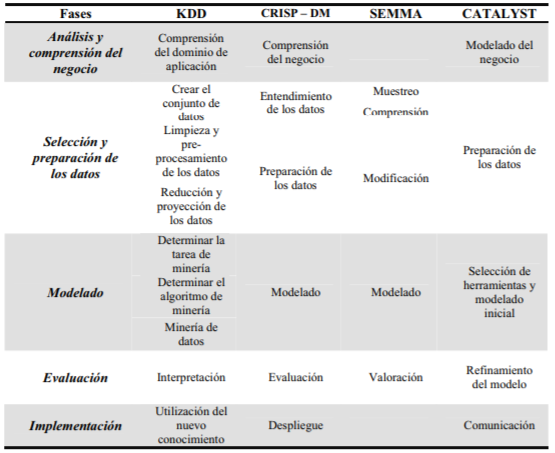
\includegraphics[width=0.8\textwidth]{recursos/ComparacionModelosDM}
	\label{fig:compMod}
\end{figure*}
\FloatBarrier


La metodología de trabajo predominante en los artículos observados de carácter educativo ha sido la metodología CRISP-DM (del inglés Cross Industry Standard Process for Data Mining) que es una metodología frecuente en el desarrollo de proyectos de minería de datos. Esta metodología indica cómo debe realizarse, mediante tareas, dichos proyectos. Esta metodología se ha utilizado en artículos como \citeA{FERNANDES2019335}, \citeA{DELEN2010498}, \citeA{SEN20129468}, \citeA{jaramillo2015aplicacion} y \citeA{chalaris2014improving}.

Según \citeA{jaramillo2015aplicacion}, en su investigación se ha seleccionado Crisp-DM por las siguientes razones: ''La metodología a utilizar es Crisp-DM ya que cada una de sus fases se encuentra claramente estructurada definiendo de tal forma las actividades y tareas que se requieren para lograr el objetivo planteado, es decir, la más completa entre las metodologías comparadas, es flexible por ende se puede hacer usos de cualquier herramienta de minería de datos'', idea ya presentada en el artículo de \cite{moine2011analisis}.

\subsection{Modelos utilizados en el desarrollo de proyectos de minería de datos en el entorno educativo}
Una vez que se ha revisado los artículos existentes, se debe abstraer la información relativa a los modelos utilizados con el objetivo de obtener un estado de la situación de dichos modelos.

En el artículo de prensa de \citeA{FERNANDES2019335}, se muestra el uso de técnicas como los métodos de clasificación y el algoritmo predictivo de GBM (Gradient Boosting Model) con el objetivo de obtener aquellas variables en el entorno del alumno, que hace que este obtenga mejores o peores resultados escolares. Este estudio, además, tiene el objetivo de aportar información útil para los representantes políticos en el ámbito educativo, el consejo escolar y los profesores con el objetivo de que estos puedan realizar políticas públicas, materiales didácticos y trabajo social para beneficiar a los estudiantes.

En el artículo de \citeA{SHAHIRI2015414} se indica que ``a priori", sin tener en cuenta la experiencia, es necesario realizar un proyecto piloto, que responda a dos preguntas en concreto. La primera pregunta que se plantea son los atributos o variables a utilizar en la investigación. La segunda pregunta planteada es sobre los métodos predictivos a utilizar. La siguiente figura \ref{fig:precMet} obtenida del artículo, muestra la precisión en la predicción de los algoritmos entre los años 2002 y 2015.

\begin{figure*}[htb]
	\centering
	\caption{Predicción en la precisión agrupada por algoritmos desde 2002 a 2015. Recuperado de \protect\citeA{SHAHIRI2015414}}
	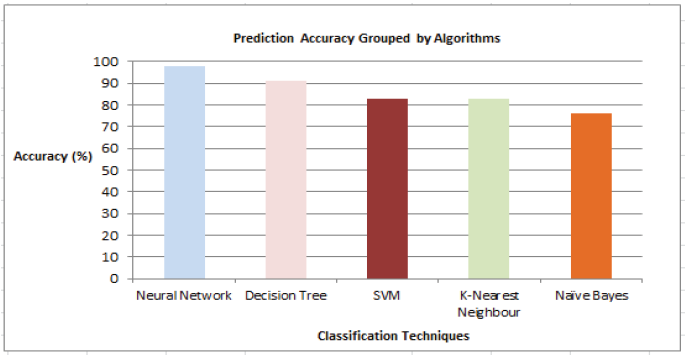
\includegraphics[width=0.8\textwidth]{recursos/PrecisionMetodos}
	\label{fig:precMet}
\end{figure*}

Teniendo en cuenta dicha figura, vemos que las redes neuronales son las que obtienen mejores resultados junto con los arboles de decisiones, lo que significa que se ajustan más a los datos. 

Los resultados obtenidos en otro artículo, concretamente el de \citeA{ASHRAF20181021}, indican que el mejor modelo para los datos propuestos ha sido obtenido utilizando el algoritmo de bosques aleatorios. Este algoritmo ha obtenido mejores resultados que otros algoritmos como los arboles de decisión o árbol aleatorio. Este articulo utiliza también datos académicos de alumnos, en este caso, pertenecientes a la Universidad Kashmir.

Para lograr los objetivos establecidos en el análisis del rendimiento académico, \citeA{ASIF2017177}, va a utilizar los arboles de decisión, Naïves Bayes, Redes Neuronales, 1-Vecino-Cercano y Bosques Aleatorios. Los mejores resultados se han obtenido utilizando el algoritmo de Naïves Bayes, obteniendo un 85\% de precisión.

En cuanto al artículo de \citeA{ADEKITAN2019e01250}, nuevamente se han utilizado algoritmos como redes neuronales, bosques aleatorios, arboles de decisión, Naïve Bayes, combinación de árboles y regresión logística. En la figura \ref{fig:compResMod} se puede observar la comparación entre los modelos.

\begin{figure*}[htb]
	\centering
	\caption{Comparación de los resultados obtenidos. Recuperado de \protect\citeA{ADEKITAN2019e01250}}
	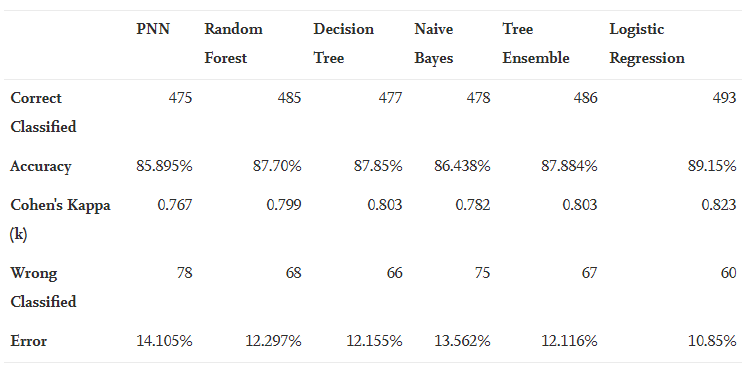
\includegraphics[width=0.8\textwidth]{recursos/ComparacionModelos}
	\label{fig:compResMod}
\end{figure*}
\FloatBarrier

En este artículo \citeA{ADEKITAN2019e01250}, se puede observar como la regresión logística obtiene la mayor precisión en los resultados. Por tanto, es capaz de clasificar correctamente los datos y, en consiguiente, obtener mejores predicciones. Otro artículo donde la regresión logística es la que mayor precisión da es el de \citeA{lehr2016use}, donde además se utilizan los algoritmos de Naïves Bayes, Bosques aleatorios, arboles de decisión y K-vecinos-cercanos.



\subsection{Herramientas analizadas para la minería de datos}
Existen diversas herramientas para realizar minería de datos, por lo tanto, se debe analizar cuales se están utilizando en los artículos estudiados e incluso se debe revisar no solo en el ámbito educativo, sino de forma general. De esta forma obtendremos las herramientas más utilizadas.

En el artículo de \citeA{rodriguez2009herramientas} se recogen algunas de las más utilizadas. Entre ellas se puede destacar SPSS Clementine, WEKA y Oracle Data Miner. Además, artículos como el de \citeA{jose2016explotacion} han utilizado R, que es un lenguaje estadístico.

R al estar orientado a la estadística, proporciona un gran número de bibliotecas y herramientas. Destaca también por la generación de gráficos estadísticos de gran calidad. Posee muchos paquetes dedicados a la graficación. Además, es una herramienta que facilita el cálculo numérico y el uso en la minería de datos. \cite{emanuel2014}

Su potencia reside fundamentalmente en que es un software gratuito y de código abierto. Como ya se ha comentado, posee un gran número de herramientas que pueden ampliarse mediante paquetes, librerías o definiendo funciones propias.

Por otro lado, RStudio es el entorno de desarrollo para R. Es también software libre y tiene la ventaja que se puede ejecutar sobre distintas plataformas (Windows, Mac y Linux).

En el artículo de \citeA{jaramillo2015aplicacion}, se ha realizado una breve comparación nuevamente entre las herramientas de WEKA, RapidMiner y Knime. De esta comparación, los autores han seleccionado la herramienta de RapidMiner para realizar las investigaciones por las siguientes características: ``posee una licencia libre, combinación de modelos, interfaz amiga, multiplataforma, empleo de técnicas, además permite aplicar varios algoritmos de minería de datos...'' \cite{jaramillo2015aplicacion}

En la figura \ref{fig:top10tools} se pueden observar las 10 herramientas más utilizadas en 2013 según Rexer Analytics. \cite{rexer2013}

\begin{figure*}[htb]
	\centering
	\caption{Herramientas más usadas. Recuperado de \protect\cite{rexer2013}}
	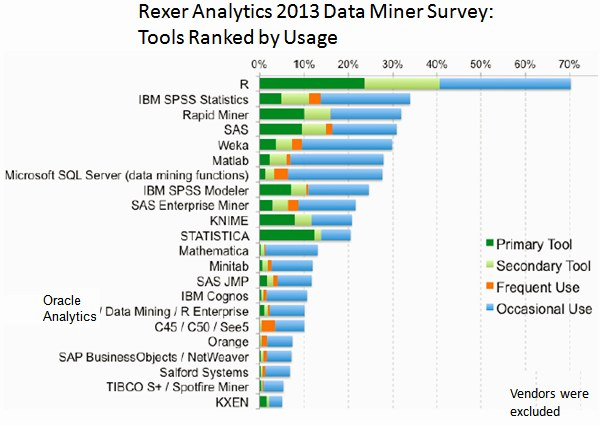
\includegraphics[width=1\textwidth]{recursos/top10tools}
	\label{fig:top10tools}
\end{figure*}
\FloatBarrier

Como se puede observar en la figura \ref{fig:top10tools}, las herramientas más utilizadas son R, IBM SPSS Statistics, RapidMiner, y también en puestos superiores se encuentra Weka.

Por otro lado, también se ha consultado la página de Gartner, que es una empresa consultora y de investigación de las tecnologías de la información y que realiza informe sobre las herramientas existentes. En la siguiente figura \ref{fig:gartner} se muestra las herramientas más usadas dividas en cuadrantes dependiendo de la habilidad necesaria para usarlas y la visión completa de estas.

\begin{figure*}[htb]
	\centering
	\caption{Plataformas de ciencia de datos y aprendizaje de máquina. Recuperado de Gartner (https://www.gartner.com)}
	\includegraphics[width=0.6\textwidth]{recursos/gartner}
	\label{fig:gartner}
\end{figure*}
\FloatBarrier

Teniendo conocimiento sobre las herramientas más utilizadas, se debe elegir una de ellas para realizar la investigación de este TFM.



\subsection{Conclusiones}
%Una vez que se ha realizado un análisis sobre la metodología utilizada y los algoritmos predictivos, además de tener en cuenta las variables utilizadas (relacionadas con el entorno del alumno), se va a realizar una investigación sobre nuevas variables que podrían incluirse en este TFM.

Teniendo en cuenta los artículos anteriores, vemos que existen metodologías, técnicas y herramientas comunes, sin embargo, dependiendo del artículo, unas técnicas obtienen mejores resultados que otras. Esto se debe al carácter de los datos. 

En cuanto a las metodologías, existen muchas investigaciones que utilizan sus propias metodologías en vez de utilizar aquellas de uso frecuente. No obstante, es importante tener claro el procedimiento a seguir.

Por otro lado, también se ha comprobado que existen un gran número de variables comunes de estudio en la mayoría de los artículos. Esto se debe a que la mayoría de los artículos tienen una gran relación, y es investigar acerca de factores que impliquen un mejor rendimiento en los alumnos. Algunas de estas variables se pueden considerar en la investigación de este TFM.

Respecto a los modelos utilizados, se han utilizado algoritmos comunes en varios artículos, y como ya se ha comentado, en ciertas ocasiones han sido más precisos que en otras. Esto se debe a los propios datos. Por tanto, en este TFM se realizan pruebas con distintos modelos y se selecciona el que mejor resultados obtenga.

Por último, en muchos artículos no se ha referenciado las herramientas utilizadas para llevar a cabo la investigación, sin embargo, se ha acudido a otras fuentes para obtener las herramientas con mayor uso. El uso de unas herramientas u otras, no es relevante, puesto que, a día de hoy, la mayoría de las herramientas satisfacen las necesidades de los investigadores, sin embargo, se debe tener en cuenta la licencia comercial, las posibles librerías, etc. que nos pueda o no proporcionar la herramienta.

%Por tanto, una vez que se ha estudiado una metodología de trabajo, y se han observado un gran número de variables relacionadas con los alumnos y con los centros, además de haber agrupado ciertos algoritmos que pueden aportar mayor información sobre los datos educativos, se va a realizar la investigación propia para resolver el problema propio de este TFM.

Por ello, se considera muy oportuno definir, en base a la literatura existente y a los métodos, técnicas, herramientas, etc. más extendidos entre la comunidad científica, una metodología para diseñar esta investigación y unas herramientas para utilizar en dicha metodología y así satisfacer las necesidades dadas.

%manage, education, data mining -> Castilla y Leon
%GIS-Based SWARA and Its Ensemble by RBF and ICA Data-Mining Techniques for Determining Suitability of Existing Schools and Site Selection of New School Buildings
%https://www.maximaformacion.es/blog-dat/como-seleccionar-las-variables-adecuadas-para-tu-modelo/



%----------------------------------------------------------------------------------------
%	MARCO TEORICO
%----------------------------------------------------------------------------------------


\chapter{Propuesta de Intervención}
\section{Justificación}
Desde la Consejería de Educación de Madrid (CEI), también se ha querido obtener información intrínseca de los datos que poseen. Una unidad integrada en la Subdirección General de Centros de Educación Secundaria ha planteado un problema que se describe a continuación.

Cada año la escolarización de alumnos en el Sistema Educativo requiere adoptar una serie de medidas que den respuesta a las necesidades de la \textbf{demanda concreta de plazas escolares del nuevo período escolar}. Estas medidas suelen centrarse en materia de nueva construcción de centros, ampliación y adaptación de sus espacios, número y distribución del profesorado, ordenación de nuevas enseñanzas y la determinación del número de unidades de escolarización en los centros.

En consecuencia, para asegurar la adecuación de dicha demanda a la oferta de escolarización del alumnado en cada nuevo curso, es indispensable que las Unidades de Gestión de la Consejería de Educación e Investigación realicen un estudio de las zonas en las que se encuentran ubicados los centros, de la diversidad de su alumnado y de las consiguientes tendencias al aumento o disminución de alumnado y de las unidades. Como resultado del oportuno análisis se ponen en marcha actuaciones para ampliar o reducir el número de grupos y plazas autorizados en cada centro, las enseñanzas a impartir y la plantilla de recursos humanos necesaria. Puede darse incluso la necesidad de agrupamientos de centros dentro de una misma localidad o distrito, o en su caso la supresión de alguno, para atender con mayor racionalidad y eficacia las distintas necesidades.

En el caso particular de la determinación de grupos o unidades de la Enseñanza Secundaria, la Unidad de Planificación de Centros Públicos, los Servicios de Inspección Educativa y la Unidad de Programas Educativos de cada Dirección de Área Territorial (DAT) deben seguir un procedimiento específico para que, dentro de su ámbito respectivo, se alcance el fin anteriormente expuesto. 

Se detalla seguidamente dicho procedimiento, contextualizándolo a la planificación para el próximo curso escolar: 


\begin{enumerate}
	\item Las DAT remiten a la Subdirección General de Centros de Educación Secundaria (SGCES) la distribución definitiva de grupos autorizados de cada centro, así como el número de alumnos matriculados, en el presente curso 2018/2019, desglosada por centros, niveles educativos, turnos y cursos de Educación Secundaria. Para los centros bilingües, se desglosa la información del total de grupos autorizados y alumnos matriculados, en grupos y alumnos de programa y sección bilingüe, y en secciones lingüísticas. Así mismo se indicará el número de grupos mixtos que el centro tenga autorizados. Para ello se utiliza un formulario, en formato Microsoft Access. 
	
	Así  mismo, en el envío,  las DAT  remiten,  en formato editable (Excel), la distribución definitiva del cupo de profesorado asignado para cada centro, desglosado por centro y por cada uno de los distintos conceptos de cupo.
	%La unidad de Secundaria envía a la Subdirección General de Centros de Educación Secundaria la distribución definitiva de grupos autorizados de cada centro, así como el número de alumnos matriculados en el presente curso, entre otra información.
	\item Las DAT realizan la propuesta de oferta educativa de cada centro para el curso 2019/2020, distribuyendo los grupos previstos por centros, niveles, turnos y cursos de Educación Secundaria. Dicha propuesta se envía a la SGCES.
	
	Para facilitar dicha labor, se envía por correo electrónico a las DAT un fichero de datos, en formato Microsoft  Access, que contiene un formulario con el listado de centros para su autorización.
	
	
	\item En la Subdirección General de Centros de Educación Secundaria, se analizan todas las propuestas recibidas. Para obtener dicha distribución de grupos autorizados, el personal debe realizar trabajos manuales de predicción. Los aspectos que se tienen en cuenta para realizar la predicción son los siguientes:
	\begin{enumerate}
		\item \textbf{Escolaridad del curso actual:}.
		\begin{itemize}
			\item Número de alumnos y grupos de un determinado centro.
			\item Número de alumnos por aula (también conocido como ratio).
			\item Matriculación de nuevos alumnos, principalmente alumnos que superan el nivel de 6º de primaria y pasan a 1º de ESO.
		\end{itemize}	
		\item \textbf{Bilingüismo} del centro. Muchos alumnos optan por centros bilingües para su mejor formación, por lo que estos centros suelen tener más demanda de alumnos.
		\item Posibilidad de creación de \textbf{nuevas zonas urbanas} cerca del centro. 
		\item Posibilidad de \textbf{apertura o cierre de centros educativos}. El cierre, por ejemplo, de un centro privado provocara una mayor tasa de matriculación de los centros contiguos. 
		\item \textbf{Porcentaje de aprobados}. Los alumnos que están ya matriculados tienen prioridad sobre los nuevos alumnos, por lo tanto, si existe una alta tasa de suspensos, quedan pocas plazas de admisión de nueva matricula.
		\item El número y la aparición de \textbf{nuevas enseñanzas}. La oferta de nuevas enseñanzas atraerá a nuevos alumnos al centro, incrementando así el número de matriculaciones.
	\end{enumerate}
	
	Para facilitar dicha labor, se envía por correo electrónico a las DAT un fichero de datos, en formato Microsoft Access, que contiene un formulario con el listado de centros para su autorización.
	\item Una vez analizadas las propuestas enviadas a la SGCES, esta se encarga de distribuir por centros los grupos de escolarización necesarios para el curso 2019/2020 y se comunicara a las DAT la distribución provisional de grupos por centro.
	\item Las DAT pueden enviar las alegaciones oportunas a la propuesta provisional.
	\item La Dirección General de Educación Infantil, Primaria y Secundaria autorizará el número de grupos y se lo comunicará a las Direcciones de Área Territorial  con el fin de que cada Área Territorial remita a los centros docentes la oferta de grupos para la escolarización del curso 2019/2020 según las fechas establecidas en la planificación del proceso de admisión. 
	
	Si se considera necesario, a fin de analizar las propuestas y observaciones remitidas, se podrán mantener reuniones de trabajo conjuntas con las Direcciones de Área Territorial.
	
	\item Una vez resuelto el proceso de admisión, en el plazo de 10 días, los Servicios de Inspección Educativa de las respectivas Direcciones de Área Territorial estudiarán con detalle los distritos y localidades con mayor o menor demanda de plazas de escolarización de la prevista. En función de estos análisis y con el fin de precisar las actuaciones para atender las necesidades del curso escolar 2019/2020, especialmente para su incidencia en 1º ESO, se remite a la Subdirección General de Centros de Educación Secundaria el informe justificativo correspondiente indicando las variaciones producidas de alumnos y grupos en los centros, por distritos o localidad, respecto de la autorización comunicada a la que se hace referencia en el apartado anterior. 
\end{enumerate}

Este procedimiento se encuentra de forma detallada en la Instrucción de la Dirección General de Educación Infantil, Primaria y Secundaria con el siguiente título: \textit{``Instrucciones de la dirección general de educación infantil, primaria y secundaria sobre la planificación del próximo curso escolar 2019/2020 en los centros públicos que imparten eso y bachillerato, creación de nuevos centros y modificación de la red, implantación y autorización de enseñanzas y propuesta de grupos''}. \cite{INSTRCONSE}

Actualmente, la Unidad de Planificación de Centros Públicos utiliza herramientas poco automatizadas  para conocer el número de alumnos y unidades, y no disponen de algoritmos predictivos que faciliten y mejoren esta labor.

Por ello, con esta investigación, lo que se persigue  es diseñar un sistema global y flexible que sea capaz de ayudar en la predicción a la Unidad de Planificación de Centros Públicos (teniendo  en cuenta los aspectos dados), otorgando así una mayor garantía en la planificación de grupos. El sistema es flexible ya permite la incorporación de nuevas variable de estudio en la predicción.

%También se va a automatizar el proceso, evitando así  las  distintas tareas mecánicas y rudimentarias.
A partir de esta investigación no solo se obtienen los mejores modelos que se ajusten a los datos, sino que se va a realizar un ``Script'' que sirva de ejemplo en el desarrollo de futuras aplicaciones. Mediante este ``Script'', que contiene un modelo entrenado -con datos anteriores-, se pueden leer archivos que contienen datos de un determinado para poder predecir, por ejemplo, los del curso siguiente a este.


\begin{comment}
\subsection{Minería de datos}
Con el objetivo de resolver el problema comentado anteriormente y satisfacer los objetivos, se plantea el uso de la ciencia de datos como proceso para descubrir relaciones entre los datos, que sean significativas. Además, se van a buscar patrones y tendencias en los datos que ayuden a la toma de decisiones.

En primer lugar, se debe tener en cuenta que la ciencia de datos aúna métodos y tecnologías que provienen del campo de las matemáticas, la estadística y la informática entre las que se pueden encontrar el análisis descriptivo o exploratorio, el aprendizaje automático (“machine learning”), el aprendizaje profundo (“Deep learning”), etc. \cite{MARIN2018}. En esta propuesta de intervención, se va a centrar en el \textbf{análisis descriptivo} y el \textbf{aprendizaje automático}.

El análisis descriptivo, como ya se ha comentado, va a ser útil para observar características de los propios datos. Entre estas características se va a poder observar cuales son las variables que más convienen al estudio por su importancia, utilizando técnicas como el análisis principal de componentes. El artículo de \citeA{COSTA2017247} incluye el apartado de pre-procesado, en el que realiza un estudio para reducir la dimensionalidad de las variables, puesto que están trabajando con un gran número de ellas.

%https://cleverdata.io/conceptos-basicos-machine-learning/
%http://publicaciones.americana.edu.co/index.php/pensamientoamericano/article/view/133
%http://disi.unal.edu.co/~eleonguz/cursos/md/presentaciones/Sesion3_AED.pdf
%https://ciberconta.unizar.es/leccion/aed/ead.pdf
El aprendizaje automático, se divide en dos áreas: el aprendizaje supervisado y el no supervisado. 

\begin{itemize}
\item El aprendizaje supervisado (o predictivos): se basa en algoritmos que intentan encontrar una función, que, dadas las entradas, asigne unas salidas adecuadas. Estos algoritmos se entrenan mediante datos históricos y de esta forma aprende a asignar salidas adecuadas en función de dichas entradas, dicho de otra forma, predice el valor de salida. A su vez, el aprendizaje supervisado se divide en regresión (si la salida es de tipo numérico) y clasificación (si la salida es del tipo categórico). \cite{Recuero2017}
\item El aprendizaje no supervisado: se utiliza en datos en los que existen variables de entrada, pero no existen variables de salida para dichas variables de entrada. Por consiguiente, solo se puede describir la estructura de los datos, para intentar conseguir algún tipo de tendencias y patrones que simplifiquen el análisis.\cite{Recuero2017} \cite{rodriguez2009herramientas}
\end{itemize}

\subsection{Lenguaje R y RStudio}
Una vez que se tienen claros los conceptos y las técnicas, se deberá elegir la herramienta de trabajo. En esta línea de investigación se va a utilizar R como lenguaje de programación y RStudio como entorno de desarrollo para R.

Como ya se ha comentado, R es un lenguaje de programación para el análisis estadístico. Al estar orientado a la estadística, proporciona un gran número de bibliotecas y herramientas. Destaca también por la generación de gráficos estadísticos de gran calidad. Posee muchos paquetes dedicados a la graficación. Además, es una herramienta que facilita el cálculo numérico y el uso en la minería de datos. \cite{emanuel2014}

Su potencia reside fundamentalmente en que es un software gratuito y de código abierto. Como ya se ha comentado, posee un gran número de herramientas que pueden ampliarse mediante paquetes, librerías o definiendo funciones propias.

Por otro lado, RStudio es el entorno de desarrollo para R. Es también software libre y tiene la ventaja que se puede ejecutar sobre distintas plataformas (Windows, Mac y Linux).
\end{comment}
% https://www.maximaformacion.es/blog-dat/que-es-r-software/





%----------------------------------------------------------------------------------------
%	VARIABLES E HIPÓTESIS
%----------------------------------------------------------------------------------------


\chapter{Diseño de Investigación}
%http://recipp.ipp.pt/bitstream/10400.22/136/3/KDD-CRISP-SEMMA.pdf
%http://www.oldemarrodriguez.com/yahoo_site_admin/assets/docs/Documento_CRISP-DM.2385037

\section{Introducción}
En un principio el proyecto comienza como parte de una necesidad que surge a la CEI. Dicha necesidad se basa en realizar explotaciones (visualizando los datos según convenga) y reportes sobre la situación actual respecto a otros años, concretamente, los últimos 10 año. \footnote{Antes del curso 2007/2008 no existe un sistema de gestión centralizado y por lo tanto no se puede hacer explotaciones}

La CEI dispone de un gran numero de bases de datos, por lo que obtener información sencilla a través de ellas resulta complejo. Por tanto, se requiere de un sistema de explotación que permita obtener el máximo valor de la información de dichas bases de datos.

 %Sin embargo, es necesario tener presente el gran numero de bases de datos que posee la Consejería de Educación e Investigación, por tanto, debido a estas demandas de explotación y al gran numero de bases de datos, es conveniente el uso de arquitecturas que nos permitan satisfacer dichas demandas.

A continuación se expone someramente la arquitectura inicial del proyecto.

	%Una de las necesidades de la Consejería de Educación e Investigación es poder visualizar los datos según convenga. Como se puede imaginar, los datos se encuentran distribuidos en diferentes tablas. Por tanto, ha sido necesario la utilización de herramientas de inteligencia de negocio para poder obtener la máxima información de los datos. 

%Para realizar esta tarea, se ha tenido que utilizar los llamados cubos OLAP, utilizando así bases de datos multidimensionales. Para ello, se ha tenido que realizar un diseño de tablas en SQL que permita modelar dichos cubos OLAP. Para ello se ha utilizado la herramienta \textit{Pentaho Schema Workbench}.

%Cuando se accedió a la informacion de la consejeria en los ultimos años, esta se remontaba a 2004. Desde este curso se comenzo a alamacenar de forma centralizada relacionada al sistema educativa y fue de forma progresiva mediante SICE, hasta 2007 no se implanto en todos los centros, por lo tanto son datos parciales (en cuanto al numero de centros). En 2007 sostenidos con fondos publicos. 

\section{Arquitectura Inicial}
Con el fin de entender conceptos posteriores, se procede a mostrar la arquitectura lógica del sistema con la que se parte inicialmente. Esta arquitectura ya está implementada y es la base del proyecto inicial y se puede observar en la figura \ref{fig:arquitecturaDWH2}
\begin{figure*}[h]
	\centering
	\caption{Arquitectura lógica del proyecto. Recuperado de la Consejería de Educación e Investigación de la Comunidad de Madrid.}
	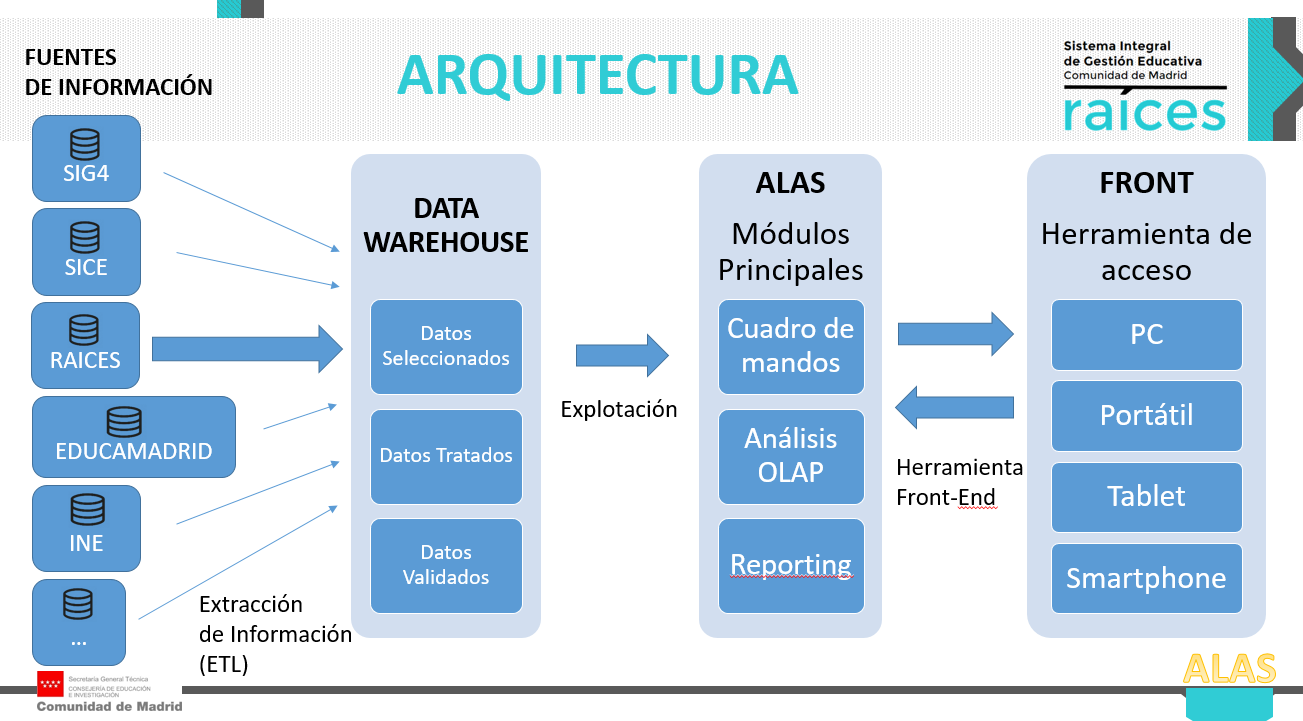
\includegraphics[width=0.8\textwidth]{recursos/arquitecturaDWH2}
	\label{fig:arquitecturaDWH2}
\end{figure*}
\FloatBarrier

%En la figura \ref{fig:arquitecturaDWH2} se muestra cuales son las fuentes de información, como se crea el ``DataWareHouse'' (que para entenderse son simplemente bases de datos con una estructura especial) y los módulos principales que se encargaran de seleccionar la información de una determinada forma para que posteriormente el usuario pueda visualizarla.
En primer lugar se tiene un gran numero de bases de datos de la CEI. A partir de los datos solicitados para realizar la explotación, se tiene que realizar la búsqueda en las tablas de estas bases de datos.

En segundo lugar, se crea un almacén de datos (Datawarehouse -DWH-), que son tablas dispuestas de una determinada forma o diseño (en este caso forma de estrella), donde se encuentran las tablas de hechos y las tablas de dimensiones. Las tablas de hechos son el corazón de un esquema en estrella, almacenan campos claves que se unen a las tablas de dimensiones, ademas incluyen métricas del negocio, contienen millones de registros. Las tablas de dimensiones son las que ofrecen mas información sobre características de las tablas de hechos, normalmente contienen pocos registros.
\begin{figure*}[h]
	\centering
	\caption{Esquema en estrella. Recuperado de http://carlospesquera.com}
	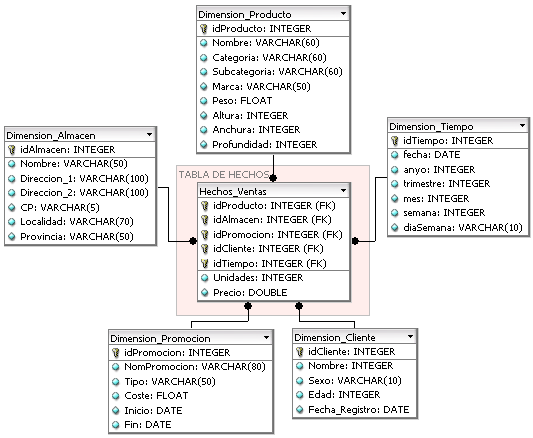
\includegraphics[width=0.8\textwidth]{recursos/Esquema_en_estrella}
	\label{fig:esquemaestrella}
\end{figure*}
\FloatBarrier

Cada tipo de diseño (en estrella o en copo de nieve), que permite realizar consultas multidimensionales, debe seleccionarse según las necesidades de los datos. Esta estructura en la base de datos es la clave para realizar los esquemas de Mondrian OLAP, conocidos como cubos de Mondrian. \cite{MONDRIAN}

\begin{figure*}[h]
	\centering
	\caption{Cubo de Mondrian. Recuperado de: https://www.businessintelligence.info}
	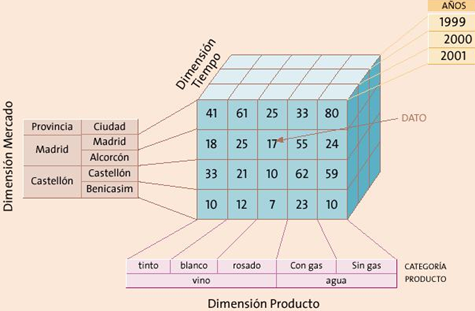
\includegraphics[width=0.8\textwidth]{recursos/modelo-dimensional-cubo}
	\label{fig:modelo-dimensional-cubo}
\end{figure*}
\FloatBarrier

Estos esquemas (que son archivos .XML) lo que hacen es ``traducir'' el diseño unidimensional de las tablas relacionales a un diseño multidimensional de forma que puedan ser entendidos por los servidores de Business Intelligence (BI). 

Para crear el esquema de Mondrian, primero se tiene que decidir cuales son las tablas de hechos y las tablas de dimensiones. Un ejemplo concreto sobre un diseño realizado en la CEI ha sido una tabla de hechos que contiene el identificador de centros, el numero de alumnos, el número de grupos, el nivel escolar, la naturaleza del centro (publico, privado o concertado), etc. La tabla de dimensiones contiene los propios valores de la tabla anterior, por ejemplo, para la columna naturaleza del centro de la tabla de hechos, existe una dimensión que contenga los valores público, privado o concertado.

Una vez que se tiene el diseño de tablas creado, ya se puede realizar la fase de extracción, transformación y carga (ETL); con la que se extraen los datos de la fuente de información, se producen las transformaciones oportunas y posteriormente dichos datos se almacenan en las tablas de hechos o dimensiones. A través de esta fase es donde se limpia los datos, eliminando las filas que no contengan todos los campos o rellenando los campos con algún valor en caso que fuera necesario.

Una vez que se tienen los datos limpios y cargados en las tablas de hechos y dimensiones, se tiene que subir el esquema al servidor y establecer una conexión con la base de datos, a partir de aquí, el trabajo es del motor OLAP del servidor, quien se encarga de traducir las opciones introducidas por el usuario en los cuadros de mandos a complejas consultas en la base de datos. 

En resumen, y a partir de los datos almacenados en el ``Datawarehouse''(DWH), la investigación que se lleva a cabo en este TFM se centra en analizar dichos datos. Pudiéndose recurrir a las fuentes de información originales para obtener nuevos datos en caso necesario. 

\section{Diseño de la minería de datos}
Una vez que se tiene claro la arquitectura principal del sistema, se establece el camino a seguir a la hora de realizar la investigación. Para ello, se utiliza la metodologia CRISP-DM. \citeA{IBMCRISP2012}

La metodología CRISP-DM tiene como objetivo orientar los proyectos de minería de datos. 
\begin{itemize}
	\item Como metodología: incluye descripciones de las fases normales de un proyecto, las tareas necesarias en cada una de las fases y una explicación de las relaciones entre las tareas.
	\item Como modelo de proceso: ofrece un resumen del ciclo vital de la minería de datos.
\end{itemize}

La metodología CRISP-DM establece un proceso genérico para satisfacer los objetivos deseados y contemplar la realización de la vigilancia e inteligencia. Este proceso se divide en distintas etapas básicas. 

\begin{figure*}[h]
\centering
\caption{Fases del ciclo de vida de CRISP-DM. Recuperado de \protect\citeA{IBMCRISP2012}.}
 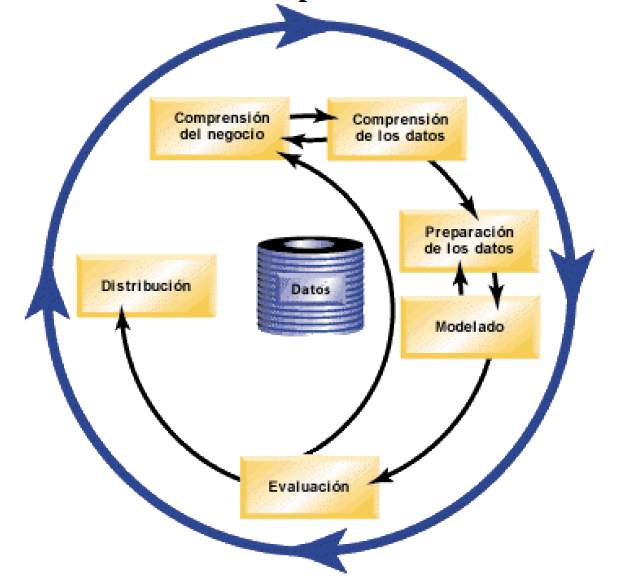
\includegraphics[width=0.6\textwidth]{recursos/CRISPCicloIBM}
\label{fig:CicloCrispDM}
\end{figure*}
\FloatBarrier
El ciclo de vida de CRISP-DM está compuesto de seis fases. La secuencia de estas no es estricta, es más, la mayoría de proyectos avanzan y retroceden entre fases si es necesario. En la figura \ref{fig:CicloCrispDM} se puede observar cada fase:

\begin{enumerate}
	\item \textbf{Comprensión del negocio.} Debe comprenderse los objetivos del negocio. Se debe realizar una descripción del problema. Por ultimo debe hacerse un plan de proyecto para alcanzar los objetivos deseados.
	\item \textbf{Comprensión de los datos.} Debe identificarse las fuentes de los datos y obtener aquellos datos relevantes para la consecución de los objetivos.
	\item \textbf{Preparación de los datos.} Conlleva el pre-procesado, la limpieza y la transformación de los datos relevantes con el objetivo de usar algoritmos de minería de datos.
	\item \textbf{Modelado.} Se debe desplegar un gran número de modelos y quedarse con aquellos que devuelvan valores óptimos para los datos utilizados.
	\item \textbf{Evaluación.} Debe evaluarse y probarse los modelos. Deben compararse entre sí y comprobar que son útiles para los datos expuestos.
	\item \textbf{Distribución.} Se realizan actividades usando los modelos seleccionados en el proceso de la toma de decisión.
\end{enumerate}

En los próximos puntos se va a describir las actividades que se realizan en cada una de estas fases.

\subsection{Comprensión del negocio}
La primera tarea a realizar en el ciclo de CRISP-DM es obtener la máxima información posible de los objetivos de esta investigación. Desde la CEI se ha comunicado la información disponible y las necesidades actuales.

Una de las necesidades de la CEI es obtener la máxima información sobre la situación actual de la educación en la comunidad de Madrid. La CEI posee una gran cantidad de datos de alumnos y centros a lo largo del tiempo. 

Por tanto, para sacar el mayor beneficio de los datos, se ha planteado el uso de herramientas y técnicas que posibiliten obtener información no solo del momento actual, sino también de la evolución a lo largo de los últimos años.

Una de las actividades que se han realizado es obtener el número de grupos y alumnos por centro, año, DAT, nivel educativo, etc.

Otra de las actividades que se realizan es obtener gráficos sobre la evolución de alumnos con necesidades especiales, alumnos de minorías étnicas e incluso porcentaje y nacionalidad de alumnos extranjeros.

\subsection{Comprensión de los datos}
Esta fase implica estudiar detalladamente los datos disponibles. Es esencial para evitar problemas inesperados durante la fase siguiente.

Para realizar esta fase, debemos tener en cuenta dos consideraciones relacionadas. La primera consideración es la identificación de necesidades de información y la segunda es la identificación de fuentes internas y externas.

\subsubsection{Identificación de necesidades de información}

Para realizar la identificación de las necesidades de información se va a partir de varios factores como son:
\begin{itemize}
	\item las demandas esperadas o manifestadas por (en este caso) una unidad de la consejería de educación.
	\item el análisis, la evolución de productos, procesos, materiales y tecnologías en el ámbito de la minería de datos educativa.
\end{itemize}

\subsubsection{Identificación de fuentes internas y externas de información}

Teniendo en cuenta las principales necesidades de información, se debe identificar las fuentes de información y recursos disponibles ya sean internos o externos a la organización. En este caso, utilizan las siguientes fuentes:
\begin{itemize}
	\item Fundamentalmente se utilizan documentos y recursos internos de la organización como: repositorios documentales, carpetas locales, bases de datos, etc.
	\item Personas con conocimientos o experiencias relacionadas con la necesidad de información. En este aspecto se realizan distintas reuniones con las personas encargadas de esta unidad de la consejería de educación. Para ello se realizarán reuniones con estos responsables. A partir de estas reuniones se obtendrán las fuentes de información.
	%\item Fuentes documentales a las que tiene acceso a la organización, ya sea en soporte físico (revistas, catálogos, etc.) como en soporte electrónico. Además, se utilizarán recursos de información en Internet (portales, noticias, redes sociales, foros, etc.). 
	\item Documentación técnica como reglamentaciones, especificaciones, propiedad industrial e intelectual o normas.
	\item Resultados de análisis existentes sobre las tendencias de futuro preferentemente en el ámbito educativo.
\end{itemize}

%\subsubsection{Búsqueda y tratamiento de la información}

La información fundamentalmente se encuentra en bases de datos internas, no obstante, se va a acceder a bases de datos externas en caso de necesidad para cumplimentar la información. 

En este aspecto, se debe recurrir a la ayuda de personas con conocimientos sobre el estado de las bases de datos. Como cualquier organización, la consejería de educación maneja grandes volúmenes de datos, por tanto, se debe tener conocimiento sobre donde se puede encontrar la información que satisfaga con las necesidades. 

El desconocimiento del estado de las bases de datos conlleva la inversión de una gran cantidad de tiempo en la búsqueda de los datos relevantes. 

De esta fase se espera localizar todos los datos que posteriormente se prepararan y se utilizaran en el modelado.

\subsection{Preparación de los datos}
Una vez que se tienen claros los datos que se utilizan, se procede a realizar la preparación para poder utilizarlos en la fase de modelado.

Algunas de las actividades que se realizan en esta fase son: la fusión de conjuntos y/o registros de datos, la selección de una muestra de un subconjunto, la agregación de registros, por contra la derivación de nuevos atributos a partir de anteriores, la eliminación o sustitución de valores en blanco o ausentes y por último la división de datos de prueba y entrenamiento.

Además, también se va a estudiar la existencia de datos perdidos y errores en estos.

Para realizar este tratamiento de datos se utilizará la técnica de ETL (extracción, transformación y carga) que consiste básicamente en obtener los datos de la fuente de origen (bases de datos, ficheros Excel, ficheros JSON, etc.), seleccionar aquellos datos que convengan al estudio, transformarlos según las necesidades que se tenga y depurarlos (evitando así datos erróneos). \cite{prakash2017etl} \cite{matos2006metodologia},\cite{gour2010improve}.
Para realizar este tratamiento, se ha va a utilizar Pentaho BI, que es un conjunto de programas libres para realizar entre otras muchas actividades, las técnicas de ETL. Concretamente, se ha utilizado la herramienta Spoon para desarrollar esta técnica. 
Una vez que se tienen los datos limpios y estructurados, se pueden realizar dos operaciones:

\begin{enumerate}
	\item  En primer lugar, se pueden almacenar dichos datos en una base de datos y seguir utilizando Pentaho BI para poder crear cuadros de mandos e informes o análisis OLAP. 
	
	\item  En segundo lugar, se puede almacenar la información en un texto plano para poder trabajar con herramientas de análisis descriptivo y predictivo. Estos análisis se realizan a través del entorno y lenguaje de programación R, que es una referencia en el ámbito de la estadística.
\end{enumerate}

\subsubsection{Análisis Exploratorio}

%El análisis predictivo (también conocido como estadísticas predictivas) se encarga de resumir los datos en bruto para que puedan ser interpretados. Estos análisis son útiles ya que permiten aprender sobre comportamientos o patrones pasados e entender cómo pueden influir en los resultados futuros. En este tipo de análisis se van a utilizar tanto métodos gráficos como medidas resumen.

La primera actividad en un análisis exploratorio es estudiar el tipo de datos de cada variable a investigar, se debe clasificar las variables según sean categóricas (dicotómicas o polinómicas) o numéricas (discretos o continuos). El tipo de datos permite decidir qué tipo de análisis estadístico utilizar.
Una vez que se tienen claro el tipo de datos utilizados, se utilizan los principales estadísticos como la media, la mediana, las desviaciones típicas, etc.
Posteriormente se va a utilizar la matriz de varianzas y covarianzas, que indicaran la variabilidad de los datos y la información sobre las posibles relaciones lineales entre las variables. 

Por otro lado, se va a estudiar la correlación de las variables mediante la matriz de correlación. Esta matriz contendrá los coeficientes de correlación.\cite{JMMarin}. La matriz de correlación, se utilizará fundamentalmente por pares entre las variables y la variable a predecir.

También se va a estudiar la matriz de correlaciones parciales, que estudia la correlación entre pares de variables eliminando el efecto de las restantes.\cite{JMMarin}

Los datos categóricos se representan en tablas de frecuencias, gráficos de barras y gráficos de sectores. Los datos numéricos se representan mediante histogramas, boxplot y diagramas QQ-Plot o Grafico Cuantil-Cuantil. \cite{Orellana2001}

Mediante el boxplot se puede observar aspectos como la posición, dispersión, asimetría, longitud de colas y los datos anómalos (outliers). 
El QQ-plot se va a utilizar para evaluar la cercanía de los datos a una distribución. \cite{Orellana2001}

%(https://www.sergas.es/gal/documentacionTecnica/docs/SaudePublica/Apli/Epidat4/Ayuda/Ayuda_Epidat_4_Analisis_descriptivo_Octubre2014.pdf)
Por otro lado, se va a complementar el análisis descriptivo mediante el aprendizaje no supervisado, donde también se extraerán otras características de los datos.

%En este apartado, se va a presentar la forma en la que se va a realizar la investigación. En primer lugar, se va a realizar un proceso ETL, posteriormente se va a realizar un análisis descriptivo mediante sus técnicas que se explicaran posteriormente, además se va a incluir técnicas de aprendizaje no supervisada en este análisis.
%Una vez que se ha realizado el análisis descriptivo, se va a realizar un análisis predictivo. En este análisis se va a utilizar técnicas de aprendizaje supervisadas.


\subsection{Modelado}
Una vez terminado el análisis descriptivo, se va a realizar un análisis predictivo. Se debe tener en cuenta, que, dentro de la ciencia de datos, existen técnicas de aprendizaje automáticas, cuyo objetivo es la construcción de un sistema que sea capaz de aprender a resolver problemas sin la intervención de un humano. \cite{MARIN2018}.

Las técnicas de aprendizaje tienen como resultado un modelo para resolver una tarea dada. Los modelos son una representación de la realidad basado en un intento descriptivo de relacionar un conjunto de variables con otro.

Los modelos predictivos son de dos tipos: regresión, que son capaces de predecir una respuesta cuantificable; y de clasificación, que son capaces de predecir respuesta categóricas.

\subsubsection{Aprendizaje automático}
%https://www.fisterra.com/mbe/investiga/10descriptiva/10descriptiva.asp#top
%http://www.uco.es/zootecniaygestion/img/pictorex/27_12_49_7.pdf
%https://machinelearningmastery.com/descriptive-statistics-examples-with-r/
%http://cms.dm.uba.ar/academico/materias/verano2015/estadisticaQ/descriptiva.pdf

El \textbf{aprendizaje supervisado} consiste en la búsqueda de patrones en datos históricos relacionando todas las variables con una especial (conocida como variable objetivo). Los algoritmos que se utilizan en el aprendizaje supervisado se encarga de buscar patrones en los datos. A este proceso se conoce como entrenamiento de los datos. Una vez que se tienen los patrones, se aplican a los datos de prueba. Los datos de entrenamiento suelen ser una selección aleatoria y única de los datos históricos de un 70\% del total. Los datos de prueba son el restante 30\%. \cite{Manguart2017}.
Algunos de los algoritmos que se utilizan son:
\begin{enumerate}
	\item \textbf{Arboles de decisión}
	
	Se basa en el descubrimiento de patrones a partir de ejemplos. Un árbol de decisión está formado por un conjunto de nodos (de decisión) y de hojas (nodos-respuesta).
	
	Los nodos están asociados a los atributos y tiene varias ramas que salen de él (dependiendo de los valores que tomen la variable asociada). Estos nodos pueden asemejarse a preguntas que, dependiendo de la respuesta que conlleve, se tomara un flujo en las ramas salientes.
	
	Los nodos respuesta están asociados a la clasificación que se desea proporcionar, devolviendo así la decisión del árbol con respecto al ejemplo de entrada utilizado.
	
	\begin{figure*}[htb]
		\centering
		\caption{Funcionamiento Árboles Decisión. Recuperado de \protect\citeA{sayad2019}}
		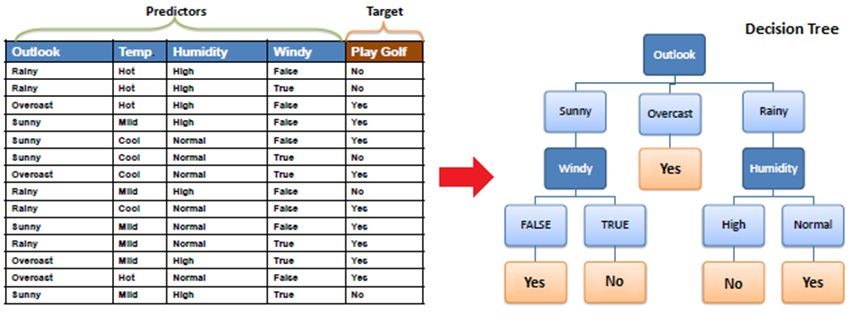
\includegraphics[width=0.8\textwidth]{recursos/arbol_decision_img1}
		\label{fig:fun_arb_dec}
	\end{figure*}
	\FloatBarrier

	
	\begin{comment}
	\item \textbf{Clasificación de Naïve Bayes}
	
	Es un algoritmo que se basa en la técnica de clasificación utilizando el teorema de Bayes.
	
	El algoritmo es capaz de agrupar un registro mediante las características de este. Para ello aplica probabilidades condicionales de las características para determinar a qué categoría pertenece. 
	
	Por ejemplo, una fruta puede considerarse una manzana si es de color rojo, redonda y tiene un determinado peso.
	
	\begin{figure*}[htb]
		\centering
		\caption{Teorema de Bayes. Recuperado de \protect\cite{uCincinnati2018}}
		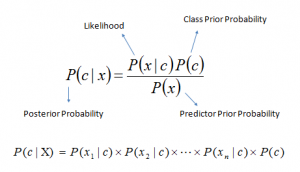
\includegraphics[width=0.6\textwidth]{recursos/BayesFormula}
		\label{fig:BayesFormula}
	\end{figure*}
	\FloatBarrier
	\end{comment}
	
	\item \textbf{Regresión Logística}
	
	Es un algoritmo de regresión que se utiliza para predecir el resultado de una variable categórica en función de las variables independientes o predictores. Para predecir el resultado, se establecen pesos en función de la puntuación dada a cada variable independiente.
	
	\item \textbf{Redes Neuronales}
	%https://www.tuinteligenciaartificial.es/las-redes-neuronales-en-la-inteligencia-artificial-explicacion-clara-y-sencilla/
	
	Las redes neuronales son un algoritmo de inteligencia artificial que se inspira en los mecanismos presentes en la naturaleza. Las neuronas envían señales eléctricas de manera fuerte o débil a otras neuronas. La combinación de todas las conexiones entre neuronas es lo que genera el conocimiento. Estas señales se envían cuando existe unos estímulos (inputs) externos a través de los sentidos. A lo largo de la vida, las neuronas aprenden que deben hacer a partir de dichos estímulos y, por lo tanto, los seres vivos aprenden a actuar ante distintas señales y situaciones. El funcionamiento de las redes neuronales en la inteligencia artificial es similar.
	
	\begin{figure*}[htb]
		\centering
		\caption{Red Neuronal. Recuperado de \protect\citeA{yepes2017}}
		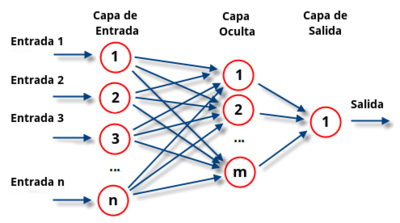
\includegraphics[width=0.6\textwidth]{recursos/RedNeuronalArtificial}
		\label {fig:RedNeuronal}
	\end{figure*}
	\FloatBarrier
	
	Como se puede observar en la figura \ref{fig:RedNeuronal}, la primera fila (con neuronas de color rojo), se conocen como nodos de entrada y son aquellos que se encargan de recoger la información. Los nodos en la gama azul son los que se conocen como nodos de salida. Los nodos situados en el medio son aquellos que se encargan de hacer el aprendizaje, y se conocen como nodos ocultos.
	
	En primer lugar, se obtiene la información a partir de los nodos de entrada, una vez que se tiene la información, se envía a las capas ocultas, que se activan o no dependiendo del aprendizaje previo. Los nodos ocultos se activan dependiendo de una serie del resultado de unas operaciones matemáticas. Si los nodos se activan, entonces enviaran la información a la siguiente capa.
	
	\item \textbf{Bosques aleatorios}
	
	Los bosques aleatorios son un método que se encarga de combinar los resultados de árboles de decisión independientes.
	
	Algunas características son:
	\begin{itemize}
		\item Gran precisión.
		\item Eficiente para grandes bases de datos.
		\item Aporta estimaciones sobre la importancia de las variables en la clasificación.
		\item Tiene un método eficaz para la estimación de los datos faltantes y mantiene la precisión cuando falta una gran parte de los datos.
	\end{itemize}
	%https://quantdare.com/random-forest-vs-simple-tree/
	%http://randomforest2013.blogspot.com/2013/05/randomforest-definicion-random-forests.html
	%https://bookdown.org/content/2031/ensambladores-random-forest-parte-i.html
	
	\item \textbf{Maquinas de Vectores Soporte (SVM)}
	Constituyen un método basado en el aprendizaje para la resolución de problemas de clasificación y regresión. Para ello, recibe unas entradas y obtienen unas salidas. Busca por tanto la curva/linea que modele la tendencia de los datos.
	
	Por ejemplo, si tenemos un anuncio en una pagina web y queremos analizar la edad y la hora del día del usuario que hace clic o no en dicho anuncio, con SVN se obtiene la "superficie optima" que delimitara el comportamiento (clic-noclic) de un determinado usuario. \cite{JANA2016}
	
		\begin{figure*}[htb]
		\centering
		\caption{Ejemplo SVM. Recuperado de \protect\citeA{JANA2016}}
		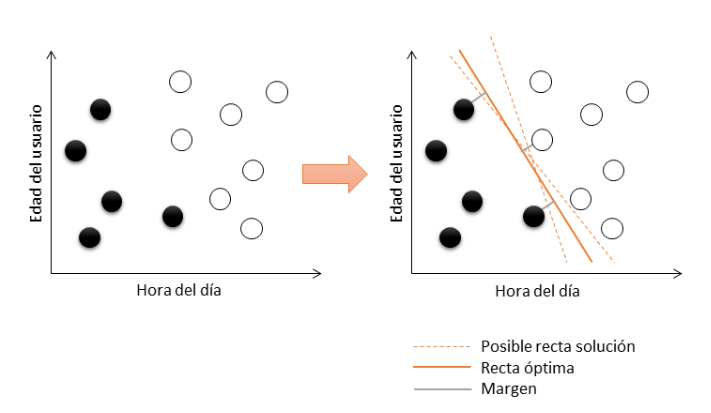
\includegraphics[width=0.6\textwidth]{recursos/SVM}
		\label {fig:SVM}
	\end{figure*}
	\FloatBarrier
	
	\item \textbf{K-Vecinos-cercanos}
	
	K-vecinos-cercanos (conocido también como K-NN) es un algoritmo de aprendizaje supervisado en el que, a partir de unos datos iniciales, es capaz de clasificar todas las nuevas instancias.
	
	La idea es que el algoritmo clasifica cada dato nuevo en el grupo que corresponda, según cual sea el grupo vecino (de los k grupos) más próximo. Por tanto, calcula la distancia del elemento nuevo a cada uno de los existentes e indica a que grupo debe permanecer este nuevo elemento según la menor distancia.
	
	\begin{figure*}[htb]
		\centering
		\caption{KNN. Recuperado de \protect\citeA{klein2018}}
		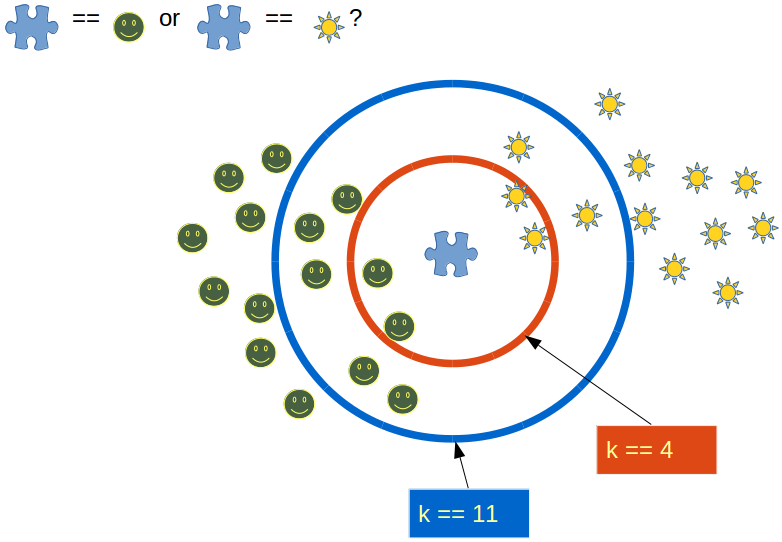
\includegraphics[width=0.6\textwidth]{recursos/k_NN}
		\label {fig:KNN}
	\end{figure*}
	\FloatBarrier
	
	
\end{enumerate}

\subsubsection{Criterio de selección}

Una vez que se han seleccionado las variables y los algoritmos a estudiar, es hora de realizar el propio modelado. Al realizar el modelado, debemos tener en cuenta que variables son mejores para este modelado. Es posible que existan variables que únicamente empeoren los resultados del modelado, por lo tanto, se deberán desestimar. Para ello se va a utilizar el criterio de Akaike (AIC). 

Este criterio indica el ajuste que tienen los datos experimentales con el modelo utilizado. Obviamente, el criterio de AIC solo tiene sentido cuando se realizan comparaciones con otros modelos (utilizando el mismo conjunto de datos). \cite{martinez2009criterio}

Cuanto menor sea el valor de este criterio, mejor se ajustan los datos al modelo. Por tanto, se deberá seleccionar el modelo que menor AIC tenga. \cite{martinez2009criterio}

\subsection{Evaluación}
En esta fase de la metodologia, se diferencian varias partes. La primera parte es la evaluación del propio modelo respecto a otros, por lo que se utilizaran las métricas de precisión. La segunda parte va a ser la evaluación de la propia Unidad de Secundaria la que evalúe los resultados de predicción obtenidos para un determinado curso con los existentes en la realidad para dicho curso.

\textbf{Métricas de precisión}
El error absoluto medio (MAE) y el error cuadrático medio (RMSE) son dos de ls métricas mas comunes utilizadas para medir la precisión de las variables continuas en los modelos de regresión.

\textbf{Error absoluto medio (MAE):} mide la magnitud promedio de los errores en un conjunto de predicciones, sin considerar su dirección. Es el promedio sobre la muestra de prueba de la diferencia absoluta entre la predicción y la observación real.
\begin{figure*}[h]
	\centering
	\caption{Fórmula de MAE. Recuperado de https://medium.com/human-in-a-machine-world/mae-and-rmse-which-metric-is-better-e60ac3bde13d}
	\includegraphics[width=0.4\textwidth]{recursos/mae}
	\label{fig:MAE}
\end{figure*}
\FloatBarrier
Error cuadrático medio (RMSE): es una regla de puntuación cuadrática que mide la magnitud promedio del error. Es la raíz cuadrada del promedio de las diferencias cuadradas entre la predicción y la observación real.
\begin{figure*}[h]
	\centering
	\caption{Fórmula de RMSE. Recuperado de https://medium.com/human-in-a-machine-world/mae-and-rmse-which-metric-is-better-e60ac3bde13d}
	\includegraphics[width=0.4\textwidth]{recursos/rmse}
	\label{fig:MAE}
\end{figure*}
\FloatBarrier

Se debe destacar que cuanto menos sea el error, más se acercan los datos predichos a la realidad.

\begin{comment}
Las métricas que se va a utilizar para obtener la precisión de los modelos son aquellas descritas en el artículo de  \citeA{COSTA2017247}, \citeA{Helal2018} y \citeA{ASHRAF20181021}. Estas métricas son frecuentes en ámbitos como la obtención de información, aprendizaje automático y otros dominios como la clasificación binaria. Dichas métricas son las siguientes:

\begin{itemize}
	\item FMeasure: es la media armónica de la precisión y recuperación de un clasificador; es decir, FMeasure = 2 * Precision * Recall / (Precision + Recall).
	\item Precision: es la fracción de verdaderos positivos entre todos los ejemplos clasificados como positivos. P= TP/(FP+TP).
	\item Recall: es la fracción de verdaderos positivos clasificados correctamente. R = TP/(FN+TP).
	\item AUC: el área bajo la característica de operación del receptor. La curva (ROC) indica la probabilidad de que un clasificador clasifique un positivo seleccionado aleatoriamente sobre un negativo. Un AUC con valor de 1 indica un perfecto clasificador, mientras que 0.5 implica que el clasificador lo hace de forma aleatoria.
\end{itemize}

Donde:
\begin{itemize}
	\item TP - Verdadero Positivo: es el número de instancias positivas clasificadas correctamente como positivas. 
	\item FP - Falso Negativo: es el número de instancias positivas clasificadas incorrectamente como negativas.
	\item FP - Falso Positivo: es el número de instancias negativas clasificadas incorrectamente como positivas.
	\item TN - Verdadero Negativo: es el número de instancias negativas clasificadas correctamente como negativas.
\end{itemize}

Estas métricas se muestran utilizando un gráfico conocido como matriz de confusión.

\end{comment}
\subsection{Distribución}
La fase de distribución considera la planificación y control de la distribución de los resultados. Debe tener en cuenta la realización de un informe final.

Respecto a la fase de distribución, se utilizan los modelos generados para predecir datos de otros cursos. Concretamente se utiliza el modelo que mayor precisión obtiene con los datos aportados.

Concretamente, los datos utilizados en la predicción son aquellos del curso 2016/2017. A partir de estos datos, se obtienen varios modelos. Una vez que se ha seleccionado el mejor modelo, ya se puede utilizar otro conjunto de datos. En este caso, el conjunto de datos a utilizar es el del curso 2017/2018.

Esta fase, por tanto, aplicada a un entorno empresarial, debería indicar que modelos deben integrarse en el sistema. En este entorno académico, simplemente se debe indicar el mejor modelo y una comparativa de todos los modelos utilizados.




 %esta no podrá salir de la CEI. Aunque se trate de datos anonimizados y agregados, se trata de datos de carácter sensible y no pueden ser distribuidos. Por tanto, dichos datos se almacenan en un gestor de bases de datos MySQL. Este gestor se encontrará en un servidor de la Consejería de Educación e Investigación. Solo se va a poder acceder a dicho servidor desde la propia sede. Es posible que los datos también se almacenen en archivos de texto plano.

\section{Herramientas utilizadas}
\subsection{Suite de Pentaho BI}
Para el desarrollo del proyecto, se tiene en cuenta la posibilidad de utilizar la herramienta de Pentaho Business Analytics, que es una suite de herramientas para la explotación de datos. Esta suite posee las herramientas que se usan y son las siguientes: Spoon, Pentaho SchemaWorkbench y Pentaho Metadata Editor.

\subsection{Lenguaje R y RStudio}
En esta línea de investigación se va a utilizar R como lenguaje de programación y RStudio como entorno de desarrollo para R.

Como ya se ha comentado, R es un lenguaje de programación para el análisis estadístico. Al estar orientado a la estadística, proporciona un gran número de bibliotecas y herramientas. Destaca también por la generación de gráficos estadísticos de gran calidad. Posee muchos paquetes dedicados a la graficación. Además, es una herramienta que facilita el cálculo numérico y el uso en la minería de datos. \cite{emanuel2014}

Su potencia reside fundamentalmente en que es un software gratuito y de código abierto. Como ya se ha comentado, posee un gran número de herramientas que pueden ampliarse mediante paquetes, librerías o definiendo funciones propias.

Por otro lado, RStudio es el entorno de desarrollo para R. Es también software libre y tiene la ventaja que se puede ejecutar sobre distintas plataformas (Windows, Mac y Linux).

\subsubsection{El Paquete \textit{Caret}}

El paquete \textbf{caret} es un conjunto de funciones que intenta agilizar el proceso de creación de modelos predictivos. El paquete contiene herramientas para: división de datos, pre-procesamiento, selección de características, ajuste del modelo mediante re-muestreo, estimación de importancia variable así como otras funcionalidades. \cite{CARET2019}





%----------------------------------------------------------------------------------------
%	METODOLOGÍA
%----------------------------------------------------------------------------------------

\chapter{ANÁLISIS DE RESULTADOS}
\section{Análisis exploratorio de datos}

Antes de comenzar con el análisis, el lector puede observar en la tabla \ref{tab:TablaVariables} del Apéndice \ref{appendix:A} las variables utilizadas en esta investigación. 

Al comienzo de esta investigación, se va a estudiar los estadísticos mas importantes de cada una de las variables. Estos estadísticos se pueden observar en la figura \ref{fig:estadisticos} del Apéndice \ref{appendix:A}.

Una vez observados los estadísticos, los vamos a representar utilizando los diagramas de caja (box-plot). Con estos diagramas vamos a observar ademas los datos atipicos (outliers). Un resumen de todos los diagramas de cajas se puede observar en la figura \ref{fig:boxplotNorm} del Apéndice \ref{appendix:A}. 

Como se puede observar en la figura \ref{fig:boxplotNorm}, existen variables que contienen valores que son atípicos. Por ejemplo, la variable "NUM\_ALUMNOS", como se puede apreciar en los estadísticos de la figura \ref{fig:estadisticos} tiene una media de 74 alumnos. No obstante, hay niveles educativos que tiene hasta casi 700 alumnos. Esto se debe a que existen centros que tienen ese numero de alumnos por nivel educativo debido a que son centros modalidades a distancia. Ocurre exactamente lo mismo con el numero de grupos "NM\_GRUPOS".

Una vez estudiado los estadísticos y los datos anómalos, se va a realizar un estudio sobre la normalidad de los datos. 

Uno de los aspectos mas importantes en el análisis exploratorio de datos es la correlación existentes entre las variables. En la figura \ref{fig:matrizcorrelaciones} se puede observar como existe una gran correlación entre las variables de numero de alumnos, numero de grupos y grupos a predecir y otra gran correlación entre la variable comedor, el carácter genérico y la naturaleza del centro. En la figura \ref{fig:mayorescorrelaciones} se pueden observar las mayores correlaciones entre variables ordenadas de mayor a menor.

Uno de los fines es obtener las variables que mejor correlacionan con la variable a predecir, en este caso "GRUPOS\_PREDECIR". En la figura \ref{fig:mayorcorrelacionpredecir} se observa como las variables ``NM\_UNIDADES" y ``NM\_ALUMNOS" son las que mayor correlación tienen con la variable a predecir. No sorprende puesto que son variables determinantes en la predicción. Vemos en la figura \ref{fig:relacionAlumnGrup} que ambas variables tienen una relación positiva que implica que si una aumenta, la otra también.






\section{Análisis predictivo}
Una vez que se realiza el análisis descriptivo, se procede a realizar el análisis predictivo.

En primer lugar, se debe tener en cuenta las variables que se van a utilizar en los modelos, para ello, se va a utilizar Random Forest como algoritmo para obtener la importancia de las variables. En la figura \ref{fig:VarImpRF} podemos del Sub-anexo \ref observar que las vas importantes a la hora de mejorar la precisión en el modelo son: NM\_UNIDADES y NM\_ALUMNOS.







%----------------------------------------------------------------------------------------
%	RESULTADOS
%----------------------------------------------------------------------------------------

%\chapter{RESULTADOS}

%----------------------------------------------------------------------------------------
%	DISCUCIÓN DE RESULTADOS
%----------------------------------------------------------------------------------------

%\chapter{DISCUSIÓN DE RESULTADOS}

%\section{Constratación de hipótesis con los resultados}

%\section{Contrastación de resultados con otros estudios similares}

%----------------------------------------------------------------------------------------
%	CONCLUSIONES
%----------------------------------------------------------------------------------------

\chapter{CONCLUSIONES Y APORTACIONES} %LISTA DE ACRONIMOS

Una vez realizado el estudio y obtenido los resultados, es hora de realizar una valoración en forma de aportaciones y conclusiones.

\section{Aportaciones de este TFM}
En esta sección se quiere hacer especial hincapié en las contribuciones de este TFM.

En primer lugar, se debe destacar las relaciones de las variables con la ratio. Estas relaciones son útiles ya que por ejemplo a partir de variables como los servicios ofertados por un centro, se puede tener la certeza que los centros que poseen dichos servicios van a ser los más demandados y, por lo tanto, se debe tener un mayor cuidado con el número de plazas ofertadas y con la sobrepoblación. Otro claro ejemplo son los centros privados, que como se muestra, su ratio suele ser más bajo (están menos sobrepoblados). 

Otra aportación que se realiza es el uso de herramientas de minería de datos para realizar la planificación de grupos en los centros educativos. Como se observa, la gran mayoría de artículos relacionados con la minería de datos en el entorno educativo, tratan sobre el rendimiento académico de forma directa. En esta investigación se ha contemplado otros aspectos del entorno educativo, como es el control de las ratios y la mejor planificación educativa.

Relacionado con la aportación anterior está el uso de modelos predictivos. En este TFM se puede observar como algunos modelos obtienen mejor predicción que otros para este conjunto de datos y en este ámbito de la educación.

Este TFM también aporta una investigación relativa a la gestión y a la planificación. Como ya se ha comentado, la mayoría de los artículos analizados se basan en la predicción del rendimiento de los alumnos y los factores que provocan dicho rendimiento (positivo o negativo), en este aspecto se abre el campo de estudio a lo referente a la planificación educativa. Destacando su importancia también en el aprendizaje y el resultado de los alumnos.

% SE APORTA UN MODELO!!!! 
% se aporta un modelo a la CEI para que esta pueda realizar nuevas planificaciones de grupos. De esta forma solo deben cargar el Excel de grupos en dicho ``Script'' y exportar los resultados con la predicción.

Por último, con este TFM, además de aportar un modelo predictivo que se ajusta a los datos y que ayude a la Unidad de Planificación de la CEI, se aportan variables que ayuden a controlar la ratio del aula y de esta forma, evitar que exista una sobrepoblación. 


%En las aportaciones tengo que intentar usar los conceptos que he utilizado en el máster. La educacion no solo consiste en dar clase, tambien hay que gestionarla. Hay que intentar hilbanar todo eso, para que sean las conclusiones

\section{Conclusiones}
Estas conclusiones se van a vincular con los objetivos propuestos en la introducción de este TFM.

La realización de este TFM tiene como objetivo principal satisfacer las necesidades de la CEI, contribuyendo a la óptima planificación de los grupos escolares para los nuevos cursos, evitando así la sobrepoblación en el aula. Para satisfacer este objetivo, se deben satisfacer unos sub objetivos establecidos. Apartado \ref{objetivos} Objetivos de la Introducción 

El primer sub objetivo consiste en la selección de variables de interés, para ello se procede a utilizar algunas de las variables propuestas a partir de la instrucción de la Unidad de Planificación \cite{INSTRCONSE}. Se tienen en cuenta inicialmente 27 variables (nombre, código y naturaleza del centro, código genérico de este, etc.), sin embargo, para el análisis predictivo se usan 11\footnote{Las variables utilizadas son: el código genérico del centro, su naturaleza, su código postal, sus servicios de transporte, comedor o bilingüismo (en caso que tengan), los niveles educativos, el curso del grupo a predecir, el número actual de unidades, la ratio de estas y el numero de unidades reales del siguiente curso}. Se eliminan todas las variables del tipo descriptivo, como por ejemplo el nombre del centro (ya que no interesa, ni tampoco su código).

El segundo sub objetivo que debe cumplirse es el estudio de la relación de estas variables para comprender el contexto de la sobrepoblación en el aula. Para ello se utiliza la correlación entre las variables. A partir de estas relaciones se observa, concretamente, los factores que hacen que la ratio aumente o disminuya, y también se observa en qué grado lo hace. 

Las variables más correlacionadas con la ratio son: el número de alumnos, la naturaleza, el servicio de comedor, el código genérico del centro y el servicio de bilingüismo. Estas variables son las que hacen que la ratio aumente o disminuya con más intensidad.

Una buena planificación en las aulas evita la superpoblación de estas y, por otra parte, también evita el gasto inadecuado de recursos. Este TFM no se centra en poner en duda la ratio de alumnos actual, sino más bien en optimizar los recursos según dicha ratio.

Para llevar a cabo esta planificación, en esta investigación se tienen en cuenta principalmente 10 variables: el código genérico del centro, su naturaleza, su código postal, sus servicios de transporte, comedor o bilingüismo (en caso que tengan), los niveles educativos, el curso del grupo a predecir, el número actual de unidades y la ratio de estas. Estas variables mayoritariamente son las que se utilizan actualmente en la CEI de la Comunidad de Madrid. Sin embargo, se proponen además nuevas variables como son la tasa de aprobados o suspensos de un determinado grupo, ya que, si la tasa de suspensos es alta, el número de matriculaciones para dicho grupo debe reducirse, y este factor condiciona claramente las futuras predicciones.

Finalmente, las variables utilizadas que realmente condicionan la predicción son las que se obtienen utilizando los algoritmos de eliminación de variables y son las siguientes: naturaleza del centro, numero de curso, número de unidades, nivel de enseñanza y ratio. Todas estas variables supeditan la sobrepoblación del aula.

Es necesario destacar la existencia de otras variables expuestas en artículos analizados previamente. Estas variables son las que están relacionadas con el entorno del centro como por ejemplo: carreteras de acceso a este, estaciones de metro cercanas, generalmente, estructuras que puedan intervenir positiva o negativamente a la tasa de matriculaciones. Estas variables son de gran interés, puesto que pueden afectar a la planificación de grupos.

El tercer sub objetivo consiste en probar distintos modelos y seleccionar aquellos con mayor precisión, por ello, se utilizan una serie de algoritmos como las redes neuronales, regresión lineal, bosques aleatorios, arboles de decisión, K-vecinos cercanos y soporte de máquinas vectoriales. De estos modelos se obtiene que el árbol de decisión es el que mejor precisión obtiene. Sin embargo, la regresión lineal obtiene resultados parecidos y su tiempo de entrenamiento es inferior.

En la tabla \ref{tab:ComparacionModelos} del Anexo \ref{appendix:B}  se puede observar una comparativa sobre la precisión y el tiempo de entrenamiento de los modelos para los datos utilizados. 

En el último sub objetivo se utiliza el algoritmo que mayor precisión aporta (arboles de decisión) con el fin de realizar predicciones con datos existentes (los 10 últimos años de la Comunidad de Madrid). Este modelo de árboles de decisión, por tanto, se aplica para el curso 2017/2018, obteniendo las predicciones para el curso 2018/2019. Estas predicciones no pueden ser contrastadas con las que realmente se producen para ese curso. Sin embargo, en reuniones posteriores, se admite que son pocos los centros que cambian el número de unidades de un curso a otro, coincidiendo con los resultados obtenidos.

Por último, se realiza una automatización del sistema de predicción, que ayuda a las personas de la CEI a planificar recursos respecto al número de unidades existentes. Se debe recordar que hasta ahora, la CEI, utiliza técnicas manuales que pueden tender a error en las predicciones. %NO QUEDA CLARO!!!! Para ello se realiza un ``Script'' en el que los usuarios introducen un archivo Microsoft Excel y obtienen las predicciones correspondientes de esos datos.

%PONER UN ULTIMO PARRAFO DONDE SE HABLE SOBRE EL MASTER Y SOBRE LA GESTION EDUCATIVA. EL MASTER ME HA APORTADO NOSEQUE Y AQUI LO UTILIZO PARA LA GESTION EDUCATIVA

Para concluir, con este TFM se han obtenido conocimientos mas allá de los adquiridos por el resto de asignaturas de este máster, con el fin también de mejorar el aprendizaje en el aula. Concretamente, este TFM se centra en nada menos que en la planificación y la gestión de la educación, parte trascendental para favorecer y mejorar la situación en el aula. Sin esta gestión y planificación, el aprendizaje dentro del aula se ve mermado. Se debe recordar que la situación actual en aula se debe gracias a la planificación y gestión de los recursos. Como docente se debe tener en cuenta el equilibrio entre el numero de grupos y los recursos, también tiene que comprenderse que, aunque la reducción del ratio es algo positivo, la mayoría de veces no se dispone de los recursos para afrontar dicha reducción.



\section{Líneas De Trabajo Futuro}
Existen ciertos puntos que se deben considerar en futuras investigaciones o en la ampliación de este trabajo.

En primer lugar, es necesario destacar el uso de otras variables que no se estudian en este TFM, por ejemplo, aspectos físicos como el acceso al centro, su comunicación con grandes vías urbanas, etc. Además, deben investigarse otras variables que no se consideran por falta de datos, como por ejemplo la tasa de aprobados o de suspensos para un grupo de un nivel determinado.

Estas variables son importantes, puesto que dependiendo de esta tasa de suspensos o aprobados, se podrán aumentar o disminuir el número de matrículas para este determinado nivel. Podría incluirse, además, el número de enseñanzas del centro, sus modalidades del bachillerato, etc.

Otras variables, como ya se comenta anteriormente son las referidas a la geolocalización del centro, su posición estratégica, y como esto puede influir al aumento de la ratio y por ende a las predicciones finales.

En segundo lugar, se deben tener en cuenta otros modelos y otros parámetros para crear los modelos como por ejemplo la regresión logística, métodos robustos, combinación de modelos, etc. Variando los parámetros de estos algoritmos se consigue una mayor precisión.

Por último, se debe tener en cuenta la realización de un Software teniendo en cuenta los modelos estudiados, que sea capaz, con una interfaz gráfica, de ayudar a los miembros de la Unidad de Planificación de Centros, sustituyendo el ``Script'' creado.




%----------------------------------------------------------------------------------------
%	RECOMENDACIONES
%----------------------------------------------------------------------------------------

%\chapter{\hspace{0.23cm}RECOMENDACIONES}

%\section{Recomendaciones}

%----------------------------------------------------------------------------------------
%	BIBLIOGRAFIA
%----------------------------------------------------------------------------------------

\bibliographystyle{apacite} % estilo de la bibliografia
\renewcommand*{\bibname}{REFERENCIAS}
\bibliography{referencias_prueba} % nombre del archivo .bib
%\addcontentsline{toc}{chapter}{REFERENCIAS}
\newpage


%----------------------------------------------------------------------------------------
%	ANEXOS
%----------------------------------------------------------------------------------------

\appendix
\clearpage
\addappheadtotoc
\appendixpage


\input{anexos.tex}


\end{document} 
